% Options for packages loaded elsewhere
\PassOptionsToPackage{unicode}{hyperref}
\PassOptionsToPackage{hyphens}{url}
\PassOptionsToPackage{dvipsnames,svgnames,x11names}{xcolor}
%
\documentclass[
]{article}
\title{Project 2}
\usepackage{etoolbox}
\makeatletter
\providecommand{\subtitle}[1]{% add subtitle to \maketitle
  \apptocmd{\@title}{\par {\large #1 \par}}{}{}
}
\makeatother
\subtitle{Computer Intensive Statistical Methods}
\author{Erling Fause Steen og Christian Oppegård Moen}
\date{08 03 2022}

\usepackage{amsmath,amssymb}
\usepackage{lmodern}
\usepackage{iftex}
\ifPDFTeX
  \usepackage[T1]{fontenc}
  \usepackage[utf8]{inputenc}
  \usepackage{textcomp} % provide euro and other symbols
\else % if luatex or xetex
  \usepackage{unicode-math}
  \defaultfontfeatures{Scale=MatchLowercase}
  \defaultfontfeatures[\rmfamily]{Ligatures=TeX,Scale=1}
\fi
% Use upquote if available, for straight quotes in verbatim environments
\IfFileExists{upquote.sty}{\usepackage{upquote}}{}
\IfFileExists{microtype.sty}{% use microtype if available
  \usepackage[]{microtype}
  \UseMicrotypeSet[protrusion]{basicmath} % disable protrusion for tt fonts
}{}
\makeatletter
\@ifundefined{KOMAClassName}{% if non-KOMA class
  \IfFileExists{parskip.sty}{%
    \usepackage{parskip}
  }{% else
    \setlength{\parindent}{0pt}
    \setlength{\parskip}{6pt plus 2pt minus 1pt}}
}{% if KOMA class
  \KOMAoptions{parskip=half}}
\makeatother
\usepackage{xcolor}
\IfFileExists{xurl.sty}{\usepackage{xurl}}{} % add URL line breaks if available
\IfFileExists{bookmark.sty}{\usepackage{bookmark}}{\usepackage{hyperref}}
\hypersetup{
  pdftitle={Project 2},
  pdfauthor={Erling Fause Steen og Christian Oppegård Moen},
  colorlinks=true,
  linkcolor={Maroon},
  filecolor={Maroon},
  citecolor={Blue},
  urlcolor={blue},
  pdfcreator={LaTeX via pandoc}}
\urlstyle{same} % disable monospaced font for URLs
\usepackage[margin=1in]{geometry}
\usepackage{color}
\usepackage{fancyvrb}
\newcommand{\VerbBar}{|}
\newcommand{\VERB}{\Verb[commandchars=\\\{\}]}
\DefineVerbatimEnvironment{Highlighting}{Verbatim}{commandchars=\\\{\}}
% Add ',fontsize=\small' for more characters per line
\usepackage{framed}
\definecolor{shadecolor}{RGB}{248,248,248}
\newenvironment{Shaded}{\begin{snugshade}}{\end{snugshade}}
\newcommand{\AlertTok}[1]{\textcolor[rgb]{0.94,0.16,0.16}{#1}}
\newcommand{\AnnotationTok}[1]{\textcolor[rgb]{0.56,0.35,0.01}{\textbf{\textit{#1}}}}
\newcommand{\AttributeTok}[1]{\textcolor[rgb]{0.77,0.63,0.00}{#1}}
\newcommand{\BaseNTok}[1]{\textcolor[rgb]{0.00,0.00,0.81}{#1}}
\newcommand{\BuiltInTok}[1]{#1}
\newcommand{\CharTok}[1]{\textcolor[rgb]{0.31,0.60,0.02}{#1}}
\newcommand{\CommentTok}[1]{\textcolor[rgb]{0.56,0.35,0.01}{\textit{#1}}}
\newcommand{\CommentVarTok}[1]{\textcolor[rgb]{0.56,0.35,0.01}{\textbf{\textit{#1}}}}
\newcommand{\ConstantTok}[1]{\textcolor[rgb]{0.00,0.00,0.00}{#1}}
\newcommand{\ControlFlowTok}[1]{\textcolor[rgb]{0.13,0.29,0.53}{\textbf{#1}}}
\newcommand{\DataTypeTok}[1]{\textcolor[rgb]{0.13,0.29,0.53}{#1}}
\newcommand{\DecValTok}[1]{\textcolor[rgb]{0.00,0.00,0.81}{#1}}
\newcommand{\DocumentationTok}[1]{\textcolor[rgb]{0.56,0.35,0.01}{\textbf{\textit{#1}}}}
\newcommand{\ErrorTok}[1]{\textcolor[rgb]{0.64,0.00,0.00}{\textbf{#1}}}
\newcommand{\ExtensionTok}[1]{#1}
\newcommand{\FloatTok}[1]{\textcolor[rgb]{0.00,0.00,0.81}{#1}}
\newcommand{\FunctionTok}[1]{\textcolor[rgb]{0.00,0.00,0.00}{#1}}
\newcommand{\ImportTok}[1]{#1}
\newcommand{\InformationTok}[1]{\textcolor[rgb]{0.56,0.35,0.01}{\textbf{\textit{#1}}}}
\newcommand{\KeywordTok}[1]{\textcolor[rgb]{0.13,0.29,0.53}{\textbf{#1}}}
\newcommand{\NormalTok}[1]{#1}
\newcommand{\OperatorTok}[1]{\textcolor[rgb]{0.81,0.36,0.00}{\textbf{#1}}}
\newcommand{\OtherTok}[1]{\textcolor[rgb]{0.56,0.35,0.01}{#1}}
\newcommand{\PreprocessorTok}[1]{\textcolor[rgb]{0.56,0.35,0.01}{\textit{#1}}}
\newcommand{\RegionMarkerTok}[1]{#1}
\newcommand{\SpecialCharTok}[1]{\textcolor[rgb]{0.00,0.00,0.00}{#1}}
\newcommand{\SpecialStringTok}[1]{\textcolor[rgb]{0.31,0.60,0.02}{#1}}
\newcommand{\StringTok}[1]{\textcolor[rgb]{0.31,0.60,0.02}{#1}}
\newcommand{\VariableTok}[1]{\textcolor[rgb]{0.00,0.00,0.00}{#1}}
\newcommand{\VerbatimStringTok}[1]{\textcolor[rgb]{0.31,0.60,0.02}{#1}}
\newcommand{\WarningTok}[1]{\textcolor[rgb]{0.56,0.35,0.01}{\textbf{\textit{#1}}}}
\usepackage{longtable,booktabs,array}
\usepackage{calc} % for calculating minipage widths
% Correct order of tables after \paragraph or \subparagraph
\usepackage{etoolbox}
\makeatletter
\patchcmd\longtable{\par}{\if@noskipsec\mbox{}\fi\par}{}{}
\makeatother
% Allow footnotes in longtable head/foot
\IfFileExists{footnotehyper.sty}{\usepackage{footnotehyper}}{\usepackage{footnote}}
\makesavenoteenv{longtable}
\usepackage{graphicx}
\makeatletter
\def\maxwidth{\ifdim\Gin@nat@width>\linewidth\linewidth\else\Gin@nat@width\fi}
\def\maxheight{\ifdim\Gin@nat@height>\textheight\textheight\else\Gin@nat@height\fi}
\makeatother
% Scale images if necessary, so that they will not overflow the page
% margins by default, and it is still possible to overwrite the defaults
% using explicit options in \includegraphics[width, height, ...]{}
\setkeys{Gin}{width=\maxwidth,height=\maxheight,keepaspectratio}
% Set default figure placement to htbp
\makeatletter
\def\fps@figure{htbp}
\makeatother
\setlength{\emergencystretch}{3em} % prevent overfull lines
\providecommand{\tightlist}{%
  \setlength{\itemsep}{0pt}\setlength{\parskip}{0pt}}
\setcounter{secnumdepth}{-\maxdimen} % remove section numbering
\usepackage[width=0.8\textwidth]{caption}
\ifLuaTeX
  \usepackage{selnolig}  % disable illegal ligatures
\fi

\begin{document}
\maketitle

{
\hypersetup{linkcolor=}
\setcounter{tocdepth}{3}
\tableofcontents
}
\hypertarget{introduction}{%
\section{Introduction}\label{introduction}}

The Tokyo rainfall dataset contain the amount of rainfall for each of the \(366\) days (including February 29.) for several years. We will consider a portion of this dataset, specifically from \(1951-1989\), such that for each day \(t\neq 60\) we have \(n_t=39\) observations and for \(t=60\), February 39, we have \(n_t=10\) observation. For each day we have the response \(y_t = 0,1,2,...,n_t\) being the amount of times the rainfall exceeded \(1\)mm over the given period, given by
\begin{equation}\label{eq:1response}
  y_t | \tau_t \sim \text{Bin}(n_t,\pi (\tau _t)), \ \ \pi(\tau_t)=\frac{\exp(\tau_t)}{1+\exp(\tau_t)}=\frac{1}{1+\exp(-\tau_t)}.
\end{equation}
Here, \(\pi(\tau_t)\) is the probability of rainfall exceeding \(1\)mm and \(\tau_t\) is the logit probability of exceedence. For this project we assume conditional independence among the \(y_t|\tau_t \ \forall t=1,2,...,366\).

We will apply a Bayesian hierarchical model to the dataset, using a random walk of order 1 (RW1) to model the trend. For the model we will implement a Markov chain Monte Carlo (MCMC) sampler for the posterior using Metropolis-Hastings (MH) and Gibbs steps for specific parameters. Then we will investigate the accuracy and computational speed of the implementation compared to the built in method \texttt{INLA} in R.

\hypertarget{problem-1}{%
\section{Problem 1}\label{problem-1}}

\hypertarget{a-display}{%
\subsection{a) Display}\label{a-display}}

In Figure \ref{fig:displayData} we see the number of times the rainfall has exceeded \(1\)mm. There seem to be fewer days in the start of the year and in the end of the year with an amount of rainfall exceeding 1 mm. This is in January and December. The number of days steadily increases until the begining of the summer which seems to be the period with the most days with an amount of rainfall over 1 mm. Then, the amount of days decreases during july and august before increasing during the autumn. There also seem to be fluctuations on a daily basis from the just mentiod trend in the data. The red dot is the observation for February 29.

\begin{Shaded}
\begin{Highlighting}[]
\FunctionTok{load}\NormalTok{(}\StringTok{"./rain.rda"}\NormalTok{)}
\NormalTok{day }\OtherTok{=}\NormalTok{ rain}\SpecialCharTok{$}\NormalTok{day}
\NormalTok{n.rain }\OtherTok{=}\NormalTok{ rain}\SpecialCharTok{$}\NormalTok{n.rain}
\NormalTok{n.years }\OtherTok{=}\NormalTok{ rain}\SpecialCharTok{$}\NormalTok{n.years}
\DocumentationTok{\#\# Plotting the data}
\FunctionTok{ggplot}\NormalTok{(}\AttributeTok{data =}\NormalTok{ rain, }\AttributeTok{mapping =} \FunctionTok{aes}\NormalTok{(}\AttributeTok{x =}\NormalTok{ day, }\AttributeTok{y =}\NormalTok{ n.rain)) }\SpecialCharTok{+} \FunctionTok{geom\_line}\NormalTok{() }\SpecialCharTok{+} \FunctionTok{xlab}\NormalTok{(}\StringTok{"Day"}\NormalTok{) }\SpecialCharTok{+}
    \FunctionTok{ylab}\NormalTok{(}\StringTok{"Number of days with more than 1mm rain"}\NormalTok{) }\SpecialCharTok{+} \FunctionTok{geom\_point}\NormalTok{(}\FunctionTok{aes}\NormalTok{(}\AttributeTok{x =}\NormalTok{ day[}\DecValTok{60}\NormalTok{],}
    \AttributeTok{y =}\NormalTok{ n.rain[}\DecValTok{60}\NormalTok{]), }\AttributeTok{colour =} \StringTok{"red"}\NormalTok{)}
\end{Highlighting}
\end{Shaded}

\begin{figure}

{\centering 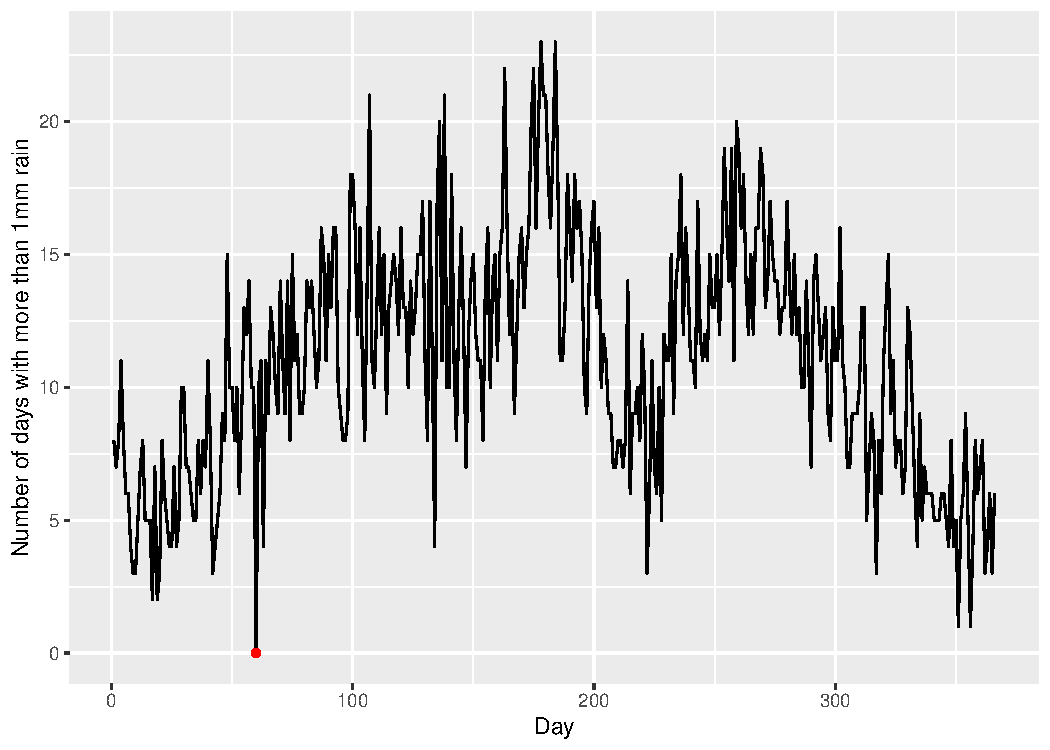
\includegraphics{Exercise-2-ny_files/figure-latex/displayData-1} 

}

\caption{The Tokyo Rainfall dataset}\label{fig:displayData}
\end{figure}

\hypertarget{b-likelihood}{%
\subsection{b) Likelihood}\label{b-likelihood}}

The likelihood of Equation \eqref{eq:1response} is given by \textcolor{red}{bc of conditional indep}
\[
\begin{array}{rl}
  L(\pi (\boldsymbol{\tau})) &= \prod_{i=1}^{T} \left(
  \begin{array}{c}
    n_t \\ y_t
  \end{array} \right)
  \pi(\tau_t)^{y_t}(1-\pi(\tau_t)^{n_t-y_t} 
  \\
  &\propto \prod_{i=1}^{T} \pi(\tau_t)^{y_t}(1-\pi(\tau_t))^{n_t-y_t} 
  \\
  &= \prod_{t=1}^{T} \left(\frac{\exp(\tau_t)}{1+\exp(\tau_t)}\right)^{y_t}
  \left( 1- \frac{\exp(\tau_t)}{1+\exp(\tau_t)}\right)^{n_t - y_t},
\end{array}
\]
where \(\boldsymbol{\tau} = (\tau_1,..., \tau_T)\), \(y_t = 1,2,...,39\) and \(n_t = 39\) for \(t \neq 60\), and \(y_t = 1,2,...,10\) and \(n_t = 10\) for \(t \neq 60\).

\hypertarget{c-posterior}{%
\subsection{c) Posterior}\label{c-posterior}}

As briefly mentioned in the introduction we need the posterior \(P(\sigma^2 | \tau, y)\) for the Gibbs step in our implementation, given by
\[
\begin{aligned}
  P(\sigma^2 | \boldsymbol{\tau}, \boldsymbol{y}) &= \frac{P(\sigma^2_u, \boldsymbol{\tau}, \boldsymbol{y})}{P(\boldsymbol{\tau}, \boldsymbol{y})}
  \\
  &\propto  P(\boldsymbol{y} | \sigma^2_u,\boldsymbol{\tau}) P(\sigma^2_u,\boldsymbol{\tau})
  \\
  &= P(\boldsymbol{y} | \sigma^2_u,\boldsymbol{\tau}) P(\tau|\sigma^2_u)P(\sigma^2_u),
\end{aligned}
\]
where \(\boldsymbol{y} = (y_1,...,y_T)^T\), \(\boldsymbol{\tau} = (\tau_1,..., \tau_T)\) and \(P(\boldsymbol{y} | \sigma^2_u,\boldsymbol{\tau}) = L(\pi( \boldsymbol{\tau}))\). Based on model assumptions mentioned in the introduction, we have \(\tau_t \sim \tau_{t-1} + u_t\) for \(u_t \stackrel{iid}{\sim} \mathcal{N}(0, \sigma_u^2)\) so that
\[
p(\boldsymbol{\tau} | \sigma_u^2) = \prod_{t=2}^{T} \frac{1}{\sigma_u} \exp\left\{ -\frac{1}{2\sigma^2_u}(\tau_t - \tau_{t-1})^2 \right\}.
\]
We place an inverse gamma prior (IG) on \(\sigma_u^2\) given by
\[
p(\sigma_u^2) = \frac{\beta^\alpha}{\Gamma(\alpha)} \left( \frac{1}{\sigma_u^2} \right)^{\alpha+1} exp\left\{ - \frac{\beta}{\sigma_u^2} \right\}.
\]
Then, the posterior is

\[
\begin{aligned}
  P(\sigma^2 | \boldsymbol{\tau}, \boldsymbol{y}) &= \underbrace{\prod_{t=1}^{T} \left(\frac{\exp(\tau_t)}{1+\exp(\tau_t)}\right)^{y_t}
  \left( 1- \frac{\exp(\tau_t)}{1+\exp(\tau_t)}\right)^{n_t - y_t}}_{\text{Constant w.r.t. }\sigma^2}\cdot \\
  &\quad \ \prod_{t=1}^{T} \frac{1}{\sigma_u} \exp\left\{ -\frac{1}{2\sigma^2_u}(\tau_t - \tau_{t-1})^2 \right\} \cdot \frac{\beta^\alpha}{\Gamma(\alpha)} \left( \frac{1}{\sigma_u^2} \right)^{\alpha+1} exp\left\{ - \frac{\beta}{\sigma_u^2} \right\}
  \\
  &\propto \prod_{t=1}^{T} \frac{1}{\sigma_u} \exp\left\{ -\frac{1}{2\sigma^2_u}(\tau_t - \tau_{t-1})^2 \right\} \cdot \frac{\beta^\alpha}{\Gamma(\alpha)} \left( \frac{1}{\sigma_u^2} \right)^{\alpha+1} exp\left\{ - \frac{\beta}{\sigma_u^2} \right\}
  \\
  &= \frac{1}{\sigma^{T-1}_u} exp\left\{ -\frac{1}{2\sigma^2_u} \boldsymbol{\tau Q \tau} \right\} \cdot \frac{\beta^\alpha}{\Gamma(\alpha)} \left( \frac{1}{\sigma_u^2} \right)^{\alpha+1} exp\left\{ - \frac{\beta}{\sigma_u^2} \right\}
  \\
  &\propto \left( \frac{1}{\sigma_u^2} \right)^{\alpha+\frac{T-1}{2} + 1} 
  exp\left\{ -\frac{1}{\sigma^2_u} \left( \frac12 \boldsymbol{\tau Q \tau} + \beta \right)  \right\}
\end{aligned}
\]
for a tri-diagonal matrix \(\boldsymbol{Q}\) with diagonal elements equal to two except first and last element which are one, and the off-diagonal elements equal to \(-1\). We recognize the posterior as the core of an inverse gamma \(\mathrm{IG}(\alpha^*, \beta^*)\) with shape \(\alpha^* = \alpha + \frac12(T-1)\) and scale \(\beta^* = \beta + \frac12 \boldsymbol{\tau Q \tau}\).

\hypertarget{sec:1d}{%
\subsection{d) Acceptance probability}\label{sec:1d}}

Let \(\mathcal{I} \subseteq \{1,2,...,366\}\) be a set of time indices, and let \(- \mathcal{I} = \{1,2,...,366\} \setminus \mathcal{I}\). Furthermore, let \(\boldsymbol{\tau}'\) denote the proposed values for \(\boldsymbol{\tau}\). The MH step needs an acceptance probability denoted \(\alpha\) for the proposed values \(\boldsymbol{\tau}'_\mathcal{I}\). By using iterative conditioning we can write the acceptance probability as
\[
 \alpha(\boldsymbol{\tau}_ \mathcal{I}| \boldsymbol{\tau}_ {-\mathcal{I}}, \sigma_u^2, \boldsymbol{y}) 
 = \text{min} \left( 1, \frac{P( \boldsymbol{\tau}'_ \mathcal{I}| \boldsymbol{\tau}_ {-\mathcal{I}}, \sigma_u^2, \boldsymbol{y})}
 {P( \boldsymbol{\tau}_ \mathcal{I}| \boldsymbol{\tau}_ {-\mathcal{I}}, \sigma_u^2, \boldsymbol{y})} 
 \frac{Q( \boldsymbol{\tau}_\mathcal{I}|\boldsymbol{\tau}_{-\mathcal{I}}, \sigma_u^2, \boldsymbol{y})}
 {Q(\boldsymbol{\tau}'_ \mathcal{I}|\boldsymbol{\tau}_{-\mathcal{I}}, \sigma_u^2, \boldsymbol{y})}
 \right),
\]
where our prior proposal distribution is \(Q(\boldsymbol{\tau}'_\mathcal{I}|\boldsymbol{\tau}_{-\mathcal{I}}, \sigma_u^2, \boldsymbol{y}) = P(\boldsymbol{\tau}'_\mathcal{I}|\boldsymbol{\tau}_{-\mathcal{I}}, \sigma_u^2)\). By considering
\[
\begin{aligned}
  P( \boldsymbol{\tau}'_ \mathcal{I}| \boldsymbol{\tau}_ {-\mathcal{I}}, \sigma_u^2, \boldsymbol{y}) &= \frac{P( \boldsymbol{\tau}'_ \mathcal{I}, \boldsymbol{\tau}_ {-\mathcal{I}}, \sigma_u^2, \boldsymbol{y})}{P( \boldsymbol{\tau}_ {-\mathcal{I}}, \sigma_u^2, \boldsymbol{y})} 
  \\
  &= \frac{P(\boldsymbol{y}| \boldsymbol{\tau}'_ \mathcal{I}, \boldsymbol{\tau}_ {-\mathcal{I}}, \sigma_u^2)P(\boldsymbol{\tau}'_ \mathcal{I}| \boldsymbol{\tau}_ {-\mathcal{I}}, \sigma_u^2)P(\boldsymbol{\tau}_ {-\mathcal{I}}, \sigma_u^2)}{P(\boldsymbol{y}| \boldsymbol{\tau}_ {-\mathcal{I}}, \sigma_u^2) P(\boldsymbol{\tau}_ {-\mathcal{I}}, \sigma_u^2)}
  \\
  &= \frac{\overbrace{P(\boldsymbol{y}| \boldsymbol{\tau}'_ \mathcal{I}, \boldsymbol{\tau}_ {-\mathcal{I}})}^{\text{Conditionally independent}} P(\boldsymbol{\tau}'_ \mathcal{I}| \boldsymbol{\tau}_ {-\mathcal{I}}, \sigma_u^2)}{P(\boldsymbol{y}| \boldsymbol{\tau}_ {-\mathcal{I}}, \sigma_u^2)}
  \\
  &= \frac{P(\boldsymbol{y}_\mathcal{I}| \boldsymbol{\tau}'_ \mathcal{I})P(\boldsymbol{y}_\mathcal{-I}| \boldsymbol{\tau}_ \mathcal{-I}) P(\boldsymbol{\tau}'_ \mathcal{I}| \boldsymbol{\tau}_ {-\mathcal{I}}, \sigma_u^2)}{P(\boldsymbol{y}| \boldsymbol{\tau}_ {-\mathcal{I}}, \sigma_u^2)}
\end{aligned}
\]
and equally
\[
  P( \boldsymbol{\tau}_ \mathcal{I}| \boldsymbol{\tau}_ {-\mathcal{I}}, \sigma_u^2, \boldsymbol{y}) 
  = 
  \frac{P(\boldsymbol{y}_\mathcal{I}| \boldsymbol{\tau}_ \mathcal{I})P(\boldsymbol{y}_\mathcal{-I}| \boldsymbol{\tau}_ \mathcal{-I}) P(\boldsymbol{\tau}_ \mathcal{I}| \boldsymbol{\tau}_ {-\mathcal{I}}, \sigma_u^2)}{P(\boldsymbol{y}| \boldsymbol{\tau}_ {-\mathcal{I}}, \sigma_u^2)}
\]
we can rewrite the acceptance probability as
\[
\begin{aligned}
  \alpha(\boldsymbol{\tau}_ \mathcal{I}| \boldsymbol{\tau}_ {-\mathcal{I}}, \sigma_u^2, \boldsymbol{y}) &= \text{min} \left( 1, \frac{{P(\boldsymbol{y}_\mathcal{I}| \boldsymbol{\tau}'_ \mathcal{I})P(\boldsymbol{y}_\mathcal{-I}| \boldsymbol{\tau}_ \mathcal{-I}) P(\boldsymbol{\tau}'_ \mathcal{I}| \boldsymbol{\tau}_ {-\mathcal{I}}, \sigma_u^2)}/{P(\boldsymbol{y}| \boldsymbol{\tau}_ {-\mathcal{I}}, \sigma_u^2)}}
  {{P(\boldsymbol{y}_\mathcal{I}| \boldsymbol{\tau}_ \mathcal{I})P(\boldsymbol{y}_\mathcal{-I}| \boldsymbol{\tau}_ \mathcal{-I}) P(\boldsymbol{\tau}_ \mathcal{I}| \boldsymbol{\tau}_ {-\mathcal{I}}, \sigma_u^2)}/{P(\boldsymbol{y}| \boldsymbol{\tau}_ {-\mathcal{I}}, \sigma_u^2)}}
  \frac{P(\boldsymbol{\tau}_\mathcal{I}|\boldsymbol{\tau}_{-\mathcal{I}}, \sigma_u^2)}{P(\boldsymbol{\tau}'_\mathcal{I}|\boldsymbol{\tau}_{-\mathcal{I}}, \sigma_u^2)} 
  \right)
  \\
  &= \text{min} \left( 1, \frac{P(\boldsymbol{y}_\mathcal{I}| \boldsymbol{\tau}'_ \mathcal{I})}{P(\boldsymbol{y}_\mathcal{I}| \boldsymbol{\tau}_ \mathcal{I})} 
  \right),
\end{aligned}
\]
which is the minimum of 1 and the ratio of likelihoods conditioned on the proposed values and the old values.

\hypertarget{sec:1e}{%
\subsection{e) Individual implementation}\label{sec:1e}}

In this section we implement an MCMC sampler for the posterior \(P(\boldsymbol{\pi}, \sigma_u^2| \boldsymbol{y})\). For the conditional prior, \(P(\tau_t | \boldsymbol{\tau}_{-t}, \sigma_u)\), we use MH steps sequentially, and for \(\sigma_u\) we use Gibbs steps. The MH steps acceptance probability for updating individual \(\tau_t\) parameters can be rewritten to improve computation time. In section \protect\hyperlink{sec:1d}{1.d)} we found that the acceptance probability is a ratio of likelihoods, which in the individual update case is given by

\begin{align}\label{eq:1eAccIndivid}
  \frac{P({y}_{t}|{\tau}'_t)}
  {P({y}_t | {\tau}_t)} 
  &= 
  \frac{\pi(\tau_t')^{y_t}(1-\pi(\tau_t'))^{n_t-y_t}}
  {\pi(\tau_t)^{y_t}(1-\pi(\tau_t))^{n_t-y_t}}              \notag \\
  &= 
  \frac{ \exp\{y_t\tau_t' - n_t \ln(1+e^{\tau'})\}}
  {\exp\{y_t\tau_t - n_t \ln(1+e^{\tau})\}}                 \notag \\
  &=
  \exp\left\{y_t(\tau'_t - \tau_t) + n_t\ln \left( \frac{1+e^{\tau}}{1+e^{\tau'}}\right)
  \right\}, 
\end{align}

for which we chose to use the logarithm seen in the function \texttt{logAccRatio}. Thus, for our random walk we accept the proposed value if \(\ln(r)\) is smaller than the logarithm of the ratio of likelihoods shown in Equation \eqref{eq:1eAccIndivid}. The \(\tau_ \mathcal{I}\) parameters for day \(\mathcal{I} = t\) and days \(- \mathcal{I}\) are multivariate Gaussian,
\[
\left(\begin{array}{l}
  {\tau}_{t} \\ 
  \boldsymbol{\tau}_{-t} 
\end{array}\right) 
\sim 
M V N\left(\left(\begin{array}{l}
{\mu}_{t} \\
\boldsymbol{\mu}_{-t}
\end{array}\right),\left(\begin{array}{ll}
{Q}_{t,t} & \mathbf{Q}_{t, -t} \\
\mathbf{Q}_{-t, t} & \mathbf{Q}_{-t,-t}
\end{array}\right)^{-1}\right).
\]
The conditional mean and precision used to draw the proposed value for \(\tau_t\) are given by
\[
\begin{aligned}
  &{\mu}_{t \mid -t}={\mu}_{t}-{Q}_{t, t}^{-1} \boldsymbol{Q}_{t,-t} \left(\boldsymbol{\tau}_{-t}-\boldsymbol{\mu}_{-t}\right) 
  = -Q_{t,t}^{-1} \boldsymbol{Q}_{t,-t}\boldsymbol{\tau}_{-t}
  \\
  &{Q}_{t \mid -t}={Q}_{t,t}.
\end{aligned}
\]

For the implementation we use the given values \(\alpha = 2\) and \(\beta = 0.05\) for the response given in Equation \eqref{eq:1response}, and we set the initial value of \(\sigma_u^2\) to be \(0.05\). Initial values for \(\tau\) are drawn from a standard normal distribution. We run the MCMC sampler for a total of \(N=50000\) iterations. In the following chunk are the functions used for the individually updating sampler followed by the chunk for which we run the sampler.

\begin{Shaded}
\begin{Highlighting}[]
\NormalTok{link }\OtherTok{=} \ControlFlowTok{function}\NormalTok{(tau) \{}
    \CommentTok{\# Expit link}
    \FunctionTok{return}\NormalTok{(}\FunctionTok{exp}\NormalTok{(tau)}\SpecialCharTok{/}\NormalTok{(}\DecValTok{1} \SpecialCharTok{+} \FunctionTok{exp}\NormalTok{(tau)))}
\NormalTok{\}}

\NormalTok{logbin }\OtherTok{=} \ControlFlowTok{function}\NormalTok{(n, y, tau) \{}
    \CommentTok{\# Remake and use this}
    \FunctionTok{return}\NormalTok{(y }\SpecialCharTok{*} \FunctionTok{log}\NormalTok{(}\DecValTok{1} \SpecialCharTok{+} \FunctionTok{exp}\NormalTok{(}\SpecialCharTok{{-}}\NormalTok{tau)) }\SpecialCharTok{{-}}\NormalTok{ (n }\SpecialCharTok{{-}}\NormalTok{ y) }\SpecialCharTok{*} \FunctionTok{log}\NormalTok{(}\DecValTok{1} \SpecialCharTok{+} \FunctionTok{exp}\NormalTok{(tau)))}
\NormalTok{\}}

\NormalTok{logAccRatio }\OtherTok{=} \ControlFlowTok{function}\NormalTok{(n, y, tauProp, tau) \{}
    \FunctionTok{return}\NormalTok{(y }\SpecialCharTok{*}\NormalTok{ (tauProp }\SpecialCharTok{{-}}\NormalTok{ tau) }\SpecialCharTok{+}\NormalTok{ n }\SpecialCharTok{*} \FunctionTok{log}\NormalTok{((}\DecValTok{1} \SpecialCharTok{+} \FunctionTok{exp}\NormalTok{(tau))}\SpecialCharTok{/}\NormalTok{(}\DecValTok{1} \SpecialCharTok{+} \FunctionTok{exp}\NormalTok{(tauProp))))}
\NormalTok{\}}

\NormalTok{mhFirst }\OtherTok{=} \ControlFlowTok{function}\NormalTok{(tau, sigma, yt, t, norm\_it, unif) \{}
    \CommentTok{\# Function to take the first MH step, i.e., for t=1}
\NormalTok{    mu\_ab }\OtherTok{=}\NormalTok{ tau[}\DecValTok{2}\NormalTok{]}
\NormalTok{    prop\_tau }\OtherTok{=}\NormalTok{ norm\_it }\SpecialCharTok{*}\NormalTok{ sigma }\SpecialCharTok{+}\NormalTok{ mu\_ab}
\NormalTok{    n }\OtherTok{=} \DecValTok{39}
    \CommentTok{\# ratio = acceptRatio(n, yt, prop\_tau, tau[t])}
\NormalTok{    ratio }\OtherTok{=} \FunctionTok{logAccRatio}\NormalTok{(}\DecValTok{39}\NormalTok{, yt, prop\_tau, tau[t])}
    \CommentTok{\# if (runif(1) \textless{} min(c(1,ratio)))\{}
    \ControlFlowTok{if}\NormalTok{ (unif }\SpecialCharTok{\textless{}} \FunctionTok{min}\NormalTok{(}\FunctionTok{c}\NormalTok{(}\DecValTok{1}\NormalTok{, ratio))) \{}
        \FunctionTok{return}\NormalTok{(}\FunctionTok{list}\NormalTok{(}\AttributeTok{tau =}\NormalTok{ prop\_tau, }\AttributeTok{accepted =} \DecValTok{1}\NormalTok{))}
\NormalTok{    \} }\ControlFlowTok{else}\NormalTok{ \{}
        \FunctionTok{return}\NormalTok{(}\FunctionTok{list}\NormalTok{(}\AttributeTok{tau =}\NormalTok{ tau[t], }\AttributeTok{accepted =} \DecValTok{0}\NormalTok{))}
\NormalTok{    \}}
\NormalTok{\}}

\NormalTok{mhLast }\OtherTok{=} \ControlFlowTok{function}\NormalTok{(tau, sigma, yt, t, norm\_it, unif) \{}
    \CommentTok{\# Function to take the last MH step, i.e., for t=366}
\NormalTok{    mu\_ab }\OtherTok{=}\NormalTok{ tau[}\DecValTok{365}\NormalTok{]}
\NormalTok{    prop\_tau }\OtherTok{=}\NormalTok{ norm\_it }\SpecialCharTok{*}\NormalTok{ sigma }\SpecialCharTok{+}\NormalTok{ mu\_ab}
    \CommentTok{\# ratio = acceptRatio(n, yt, prop\_tau, tau[t])}
\NormalTok{    ratio }\OtherTok{=} \FunctionTok{logAccRatio}\NormalTok{(}\DecValTok{39}\NormalTok{, yt, prop\_tau, tau[t])}
    \ControlFlowTok{if}\NormalTok{ (unif }\SpecialCharTok{\textless{}} \FunctionTok{min}\NormalTok{(}\FunctionTok{c}\NormalTok{(}\DecValTok{1}\NormalTok{, ratio))) \{}
        \FunctionTok{return}\NormalTok{(}\FunctionTok{list}\NormalTok{(}\AttributeTok{tau =}\NormalTok{ prop\_tau, }\AttributeTok{accepted =} \DecValTok{1}\NormalTok{))}
\NormalTok{    \} }\ControlFlowTok{else}\NormalTok{ \{}
        \FunctionTok{return}\NormalTok{(}\FunctionTok{list}\NormalTok{(}\AttributeTok{tau =}\NormalTok{ tau[t], }\AttributeTok{accepted =} \DecValTok{0}\NormalTok{))}
\NormalTok{    \}}
\NormalTok{\}}

\NormalTok{mcmcIndivid }\OtherTok{=} \ControlFlowTok{function}\NormalTok{(N, dt, }\AttributeTok{sigma0 =} \FloatTok{0.05}\NormalTok{) \{}
    \CommentTok{\# Allocate memory}
\NormalTok{    Ttot }\OtherTok{=} \DecValTok{366}
\NormalTok{    tau }\OtherTok{=} \FunctionTok{matrix}\NormalTok{(}\ConstantTok{NA}\NormalTok{, }\AttributeTok{nrow =}\NormalTok{ N, }\AttributeTok{ncol =}\NormalTok{ Ttot)}
\NormalTok{    sigma }\OtherTok{=} \FunctionTok{numeric}\NormalTok{(}\AttributeTok{length =}\NormalTok{ N)}
\NormalTok{    tau\_i }\OtherTok{=} \FunctionTok{numeric}\NormalTok{(}\AttributeTok{length =}\NormalTok{ Ttot)}
\NormalTok{    normMat }\OtherTok{=} \FunctionTok{matrix}\NormalTok{(}\FunctionTok{rep}\NormalTok{(}\FunctionTok{rnorm}\NormalTok{(Ttot), N), }\AttributeTok{nrow =}\NormalTok{ N, }\AttributeTok{ncol =}\NormalTok{ Ttot)}
    \CommentTok{\# unifMat = matrix(rep(runif(Ttot), N), nrow=N, ncol=Ttot)}
\NormalTok{    unifMat }\OtherTok{=} \FunctionTok{matrix}\NormalTok{(}\FunctionTok{rep}\NormalTok{(}\FunctionTok{log}\NormalTok{(}\FunctionTok{runif}\NormalTok{(Ttot)), N), }\AttributeTok{nrow =}\NormalTok{ N, }\AttributeTok{ncol =}\NormalTok{ Ttot)  }\CommentTok{\# log uniform}

    \CommentTok{\# Find init vals}
\NormalTok{    tau[}\DecValTok{1}\NormalTok{, ] }\OtherTok{=} \FunctionTok{rnorm}\NormalTok{(Ttot)  }\CommentTok{\# init tau drawn from normal distr.}
\NormalTok{    sigma[}\DecValTok{1}\NormalTok{] }\OtherTok{=}\NormalTok{ sigma0}

    \CommentTok{\# Run mcmc for N iterations}
\NormalTok{    accepted }\OtherTok{=} \DecValTok{0}
    \ControlFlowTok{for}\NormalTok{ (i }\ControlFlowTok{in} \DecValTok{2}\SpecialCharTok{:}\NormalTok{N) \{}
\NormalTok{        tau\_i }\OtherTok{=}\NormalTok{ tau[i }\SpecialCharTok{{-}} \DecValTok{1}\NormalTok{, ]}
\NormalTok{        sigma\_i }\OtherTok{=} \FunctionTok{sqrt}\NormalTok{(sigma[i }\SpecialCharTok{{-}} \DecValTok{1}\NormalTok{])}

        \CommentTok{\# Take first MH step for t=1}
\NormalTok{        mhStep }\OtherTok{=} \FunctionTok{mhFirst}\NormalTok{(tau\_i, sigma\_i, n.rain[}\DecValTok{1}\NormalTok{], }\DecValTok{1}\NormalTok{, normMat[i, }\DecValTok{1}\NormalTok{], unifMat[i,}
            \DecValTok{1}\NormalTok{])}
\NormalTok{        tau\_i[}\DecValTok{1}\NormalTok{] }\OtherTok{=}\NormalTok{ mhStep}\SpecialCharTok{$}\NormalTok{tau}
\NormalTok{        accepted }\OtherTok{=}\NormalTok{ accepted }\SpecialCharTok{+}\NormalTok{ mhStep}\SpecialCharTok{$}\NormalTok{accepted}

        \CommentTok{\# Perform MH steps for 1\textless{}t\textless{}366}
        \ControlFlowTok{for}\NormalTok{ (t }\ControlFlowTok{in} \DecValTok{2}\SpecialCharTok{:}\NormalTok{(Ttot }\SpecialCharTok{{-}} \DecValTok{1}\NormalTok{)) \{}
\NormalTok{            mu\_ab }\OtherTok{=} \DecValTok{1}\SpecialCharTok{/}\DecValTok{2} \SpecialCharTok{*}\NormalTok{ (tau\_i[t }\SpecialCharTok{{-}} \DecValTok{1}\NormalTok{] }\SpecialCharTok{+}\NormalTok{ tau\_i[t }\SpecialCharTok{+} \DecValTok{1}\NormalTok{])}
\NormalTok{            prop\_tau }\OtherTok{=}\NormalTok{ normMat[i, t] }\SpecialCharTok{*}\NormalTok{ sigma\_i}\SpecialCharTok{/}\DecValTok{2} \SpecialCharTok{+}\NormalTok{ mu\_ab}
\NormalTok{            ratio }\OtherTok{=} \FunctionTok{logAccRatio}\NormalTok{(n.years[t], n.rain[t], prop\_tau, tau\_i[t])}
            \ControlFlowTok{if}\NormalTok{ (unifMat[i, t] }\SpecialCharTok{\textless{}} \FunctionTok{min}\NormalTok{(}\FunctionTok{c}\NormalTok{(}\DecValTok{1}\NormalTok{, ratio))) \{}
\NormalTok{                tau\_i[t] }\OtherTok{=}\NormalTok{ prop\_tau}
\NormalTok{                accepted }\OtherTok{=}\NormalTok{ accepted }\SpecialCharTok{+} \DecValTok{1}
\NormalTok{            \}}
            \CommentTok{\# else\{tau[i,t] = tau\_i[t]\}}
\NormalTok{        \}}

        \CommentTok{\# Take last MH step for t=366}
\NormalTok{        mhStep }\OtherTok{=} \FunctionTok{mhLast}\NormalTok{(tau\_i, sigma\_i, dt}\SpecialCharTok{$}\NormalTok{n.rain[}\DecValTok{366}\NormalTok{], }\DecValTok{1}\NormalTok{, normMat[i, }\DecValTok{366}\NormalTok{], unifMat[i,}
            \DecValTok{366}\NormalTok{])}
\NormalTok{        tau\_i[}\DecValTok{366}\NormalTok{] }\OtherTok{=}\NormalTok{ mhStep}\SpecialCharTok{$}\NormalTok{tau}
\NormalTok{        tau[i, ] }\OtherTok{=}\NormalTok{ tau\_i}
\NormalTok{        accepted }\OtherTok{=}\NormalTok{ accepted }\SpecialCharTok{+}\NormalTok{ mhStep}\SpecialCharTok{$}\NormalTok{accepted}

        \CommentTok{\# Squared diff. of tau vec.  tQt = sum((tau[i,{-}Ttot] {-} tau[i,{-}1])\^{}2) \#}
        \CommentTok{\# this sim tau vals.}
\NormalTok{        tQt }\OtherTok{=} \FunctionTok{sum}\NormalTok{(}\FunctionTok{diff}\NormalTok{(tau[i, ])}\SpecialCharTok{\^{}}\DecValTok{2}\NormalTok{)  }\CommentTok{\# this sim tau vals.}

        \CommentTok{\# Gibbs step (Draw from IG)}
\NormalTok{        sigma[i] }\OtherTok{=} \DecValTok{1}\SpecialCharTok{/}\FunctionTok{rgamma}\NormalTok{(}\DecValTok{1}\NormalTok{, }\AttributeTok{shape =} \DecValTok{2} \SpecialCharTok{+}\NormalTok{ (Ttot }\SpecialCharTok{{-}} \DecValTok{1}\NormalTok{)}\SpecialCharTok{/}\DecValTok{2}\NormalTok{, }\AttributeTok{scale =} \FloatTok{0.05} \SpecialCharTok{+} \FloatTok{0.5} \SpecialCharTok{*}\NormalTok{ tQt)  }\CommentTok{\# Gibbs inline}

        \FunctionTok{setTxtProgressBar}\NormalTok{(pb, i)}
\NormalTok{    \}}
    \FunctionTok{close}\NormalTok{(pb)}
    \FunctionTok{return}\NormalTok{(}\FunctionTok{list}\NormalTok{(}\AttributeTok{tau =}\NormalTok{ tau, }\AttributeTok{sigma =}\NormalTok{ sigma, }\AttributeTok{accProb =}\NormalTok{ accepted}\SpecialCharTok{/}\NormalTok{(N }\SpecialCharTok{*}\NormalTok{ Ttot)))}
\NormalTok{\}}
\end{Highlighting}
\end{Shaded}

\begin{Shaded}
\begin{Highlighting}[]
\NormalTok{a }\OtherTok{=} \DecValTok{0}
\NormalTok{Q }\OtherTok{=} \FunctionTok{triDiag}\NormalTok{(}\AttributeTok{diagonal =} \DecValTok{2}\NormalTok{, }\AttributeTok{upper =} \SpecialCharTok{{-}}\DecValTok{1}\NormalTok{, }\AttributeTok{lower =} \SpecialCharTok{{-}}\DecValTok{1}\NormalTok{, }\AttributeTok{nrow =} \DecValTok{366}\NormalTok{)}
\NormalTok{Q[}\DecValTok{1}\NormalTok{, }\DecValTok{1}\NormalTok{] }\OtherTok{=} \DecValTok{1}
\NormalTok{Q[}\DecValTok{366}\NormalTok{, }\DecValTok{366}\NormalTok{] }\OtherTok{=} \DecValTok{1}

\FunctionTok{set.seed}\NormalTok{(}\DecValTok{321}\NormalTok{)}
\NormalTok{N }\OtherTok{=} \DecValTok{50000}
\NormalTok{pb }\OtherTok{=} \FunctionTok{txtProgressBar}\NormalTok{(}\AttributeTok{min =} \DecValTok{0}\NormalTok{, }\AttributeTok{max =}\NormalTok{ N, }\AttributeTok{initial =} \DecValTok{0}\NormalTok{)}
\NormalTok{ptm }\OtherTok{=} \FunctionTok{proc.time}\NormalTok{()}
\NormalTok{results }\OtherTok{=} \FunctionTok{mcmcIndivid}\NormalTok{(N, rain)}
\end{Highlighting}
\end{Shaded}

\begin{verbatim}
## ================================================================================
\end{verbatim}

\begin{Shaded}
\begin{Highlighting}[]
\NormalTok{time }\OtherTok{=} \FunctionTok{proc.time}\NormalTok{() }\SpecialCharTok{{-}}\NormalTok{ ptm}
\NormalTok{time}
\end{Highlighting}
\end{Shaded}

\begin{verbatim}
##    user  system elapsed 
##   39.89    0.18   40.06
\end{verbatim}

In the printout we see that computation time was 40.06. The following chunk contain functions that compute some sought values and make desired figures.

\begin{Shaded}
\begin{Highlighting}[]
\NormalTok{CImean }\OtherTok{=} \ControlFlowTok{function}\NormalTok{(p) \{}
    \CommentTok{\# Computes mean and upper,lower quantiles of vector.}
    \FunctionTok{c}\NormalTok{(}\AttributeTok{mean =} \FunctionTok{mean}\NormalTok{(p), }\FunctionTok{quantile}\NormalTok{(p, }\AttributeTok{probs =} \FunctionTok{c}\NormalTok{(}\FloatTok{0.025}\NormalTok{, }\FloatTok{0.975}\NormalTok{)))}
\NormalTok{\}}

\NormalTok{plotTAH }\OtherTok{=} \ControlFlowTok{function}\NormalTok{(p, }\AttributeTok{hcol =} \StringTok{"cyan3"}\NormalTok{, }\AttributeTok{xlab =} \StringTok{""}\NormalTok{, }\AttributeTok{ylab =} \StringTok{""}\NormalTok{, }\AttributeTok{burn =} \DecValTok{3000}\NormalTok{) \{}
    \CommentTok{\# Plots trace, autocorr and hist of probs}
\NormalTok{    l }\OtherTok{=} \FunctionTok{quantile}\NormalTok{(p, }\AttributeTok{probs =} \FloatTok{0.025}\NormalTok{)}
\NormalTok{    u }\OtherTok{=} \FunctionTok{quantile}\NormalTok{(p, }\AttributeTok{probs =} \FloatTok{0.975}\NormalTok{)}
    \FunctionTok{plot}\NormalTok{(p, }\AttributeTok{type =} \StringTok{"l"}\NormalTok{, }\AttributeTok{xlab =} \StringTok{"Iterations"}\NormalTok{, }\AttributeTok{ylab =} \StringTok{"Probability"}\NormalTok{)}
    \FunctionTok{abline}\NormalTok{(}\AttributeTok{h =} \FunctionTok{mean}\NormalTok{(p), }\AttributeTok{col =} \StringTok{"red"}\NormalTok{)}
    \FunctionTok{abline}\NormalTok{(}\AttributeTok{v =}\NormalTok{ burn, }\AttributeTok{lty =} \DecValTok{2}\NormalTok{, }\AttributeTok{col =} \StringTok{"gray"}\NormalTok{)}
    \FunctionTok{acf}\NormalTok{(p, }\AttributeTok{main =} \StringTok{""}\NormalTok{)}
    \FunctionTok{hist}\NormalTok{(p, }\AttributeTok{nclass =} \DecValTok{200}\NormalTok{, }\AttributeTok{prob =}\NormalTok{ T, }\AttributeTok{main =} \StringTok{""}\NormalTok{, }\AttributeTok{xlab =} \StringTok{"Probability"}\NormalTok{, }\AttributeTok{xlim =} \FunctionTok{c}\NormalTok{(l }\SpecialCharTok{{-}}
        \FloatTok{0.01}\NormalTok{, u }\SpecialCharTok{+} \FloatTok{0.01}\NormalTok{))}
    \FunctionTok{abline}\NormalTok{(}\AttributeTok{v =}\NormalTok{ l, }\AttributeTok{col =}\NormalTok{ hcol)}
    \FunctionTok{abline}\NormalTok{(}\AttributeTok{v =}\NormalTok{ u, }\AttributeTok{col =}\NormalTok{ hcol)}
\NormalTok{\}}
\NormalTok{pSeq }\OtherTok{=} \FunctionTok{apply}\NormalTok{(results}\SpecialCharTok{$}\NormalTok{tau, }\DecValTok{2}\NormalTok{, link)}
\end{Highlighting}
\end{Shaded}

\begin{Shaded}
\begin{Highlighting}[]
\FunctionTok{par}\NormalTok{(}\AttributeTok{mfrow =} \FunctionTok{c}\NormalTok{(}\DecValTok{3}\NormalTok{, }\DecValTok{3}\NormalTok{))}
\FunctionTok{plotTAH}\NormalTok{(pSeq[, }\DecValTok{1}\NormalTok{])}
\FunctionTok{plotTAH}\NormalTok{(pSeq[, }\DecValTok{201}\NormalTok{])}
\FunctionTok{plotTAH}\NormalTok{(pSeq[, }\DecValTok{366}\NormalTok{])}
\end{Highlighting}
\end{Shaded}

\begin{figure}

{\centering 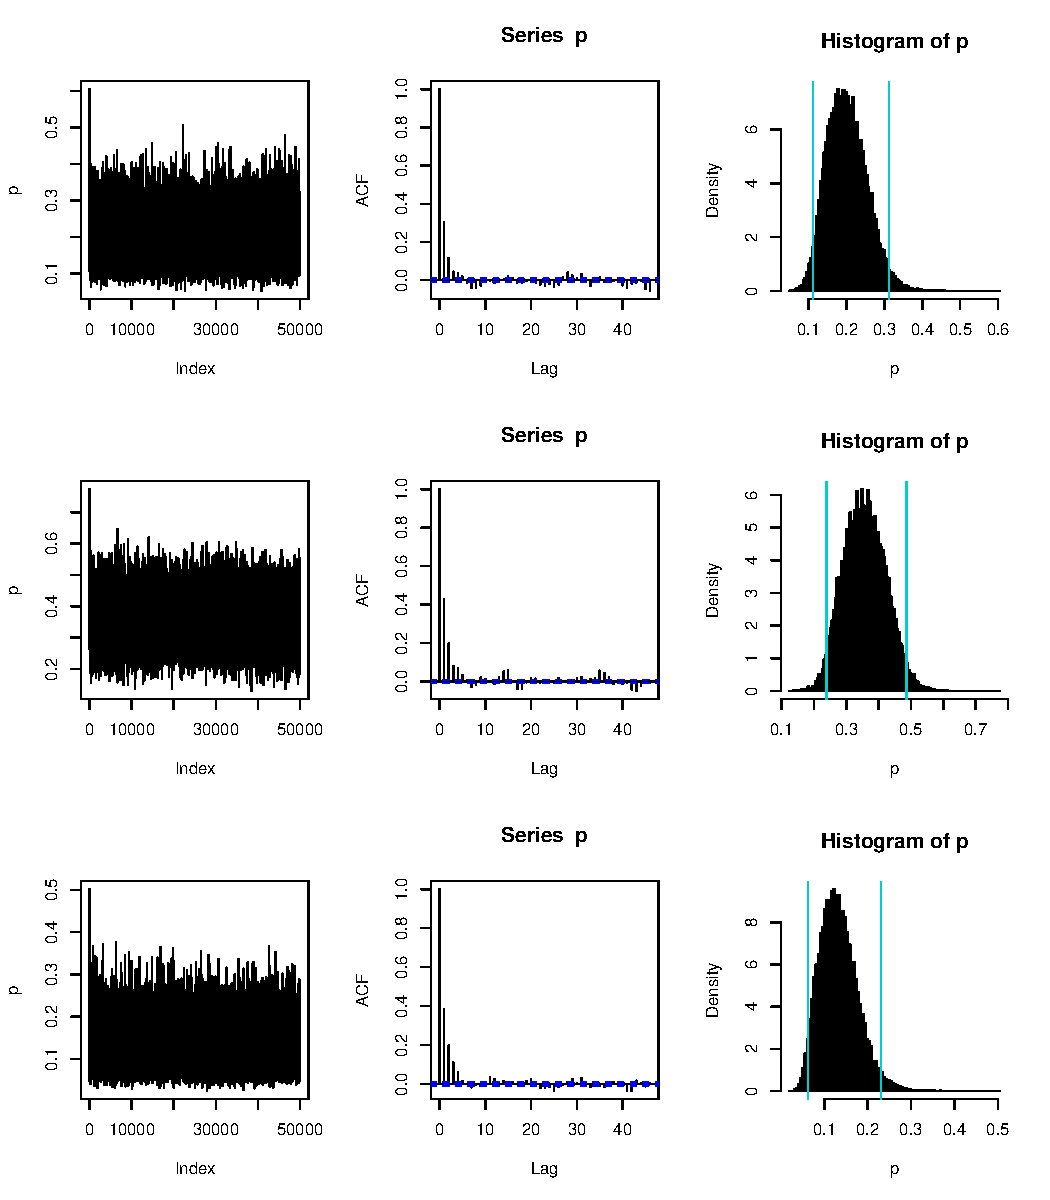
\includegraphics[width=0.9\linewidth]{Exercise-2-ny_files/figure-latex/1eDisplay-1} 

}

\caption{Traceplot, autocorrelation and histogram plots for $\pi(\tau_1), \pi(\tau_{201})$ and $\pi(\tau_{366})$ from top to bottom.}\label{fig:1eDisplay}
\end{figure}

The vertical red line in the trace plots to the left in Figure \ref{fig:1eDisplay} show the mean of \(\pi(\tau_t)\) over all \(50000\) iterations, for \(t = 1, 201, 366\). The horizontal blue line is at the \(3000^{nd}\) iteration. The vertical blue lines in the histogram plot show the \(95\%\) credible intervals for \(\pi(\tau_t)\). The traceplot bares resemblance to that of a random walk for all \(\tau_t\) after approximately the \(3000^{nd}\) iteration. We notice a decrease in autocorrelation and the histogram show that \(\pi(\tau_t)\) seem normally distributed.

\begin{Shaded}
\begin{Highlighting}[]
\NormalTok{pSeqCI }\OtherTok{=} \FunctionTok{apply}\NormalTok{(pSeq, }\DecValTok{2}\NormalTok{, CImean)  }\CommentTok{\# Compute mean and credibility interval}

\CommentTok{\# Burn}
\NormalTok{burn }\OtherTok{=} \DecValTok{3000}
\NormalTok{resultsB }\OtherTok{=}\NormalTok{ results}
\NormalTok{resultsB}\SpecialCharTok{$}\NormalTok{tau }\OtherTok{=}\NormalTok{ results}\SpecialCharTok{$}\NormalTok{tau[burn}\SpecialCharTok{:}\NormalTok{N, ]}
\NormalTok{resultsB}\SpecialCharTok{$}\NormalTok{sigma }\OtherTok{=}\NormalTok{ results}\SpecialCharTok{$}\NormalTok{sigma[burn}\SpecialCharTok{:}\NormalTok{N]}
\NormalTok{pSeqB }\OtherTok{=}\NormalTok{ pSeq[burn}\SpecialCharTok{:}\NormalTok{N, ]}
\NormalTok{pSeqCIB }\OtherTok{=} \FunctionTok{apply}\NormalTok{(pSeqB, }\DecValTok{2}\NormalTok{, CImean)  }\CommentTok{\# Compute mean and CI}
\NormalTok{ciAndMean }\OtherTok{=} \FunctionTok{rbind}\NormalTok{((pSeqCI[, }\DecValTok{1}\NormalTok{]), (pSeqCIB[, }\DecValTok{1}\NormalTok{]), (pSeqCI[, }\DecValTok{201}\NormalTok{]), (pSeqCIB[, }\DecValTok{201}\NormalTok{]),}
\NormalTok{    (pSeqCI[, }\DecValTok{366}\NormalTok{]), (pSeqCIB[, }\DecValTok{366}\NormalTok{]), }\FunctionTok{CImean}\NormalTok{(results}\SpecialCharTok{$}\NormalTok{sigma), }\FunctionTok{CImean}\NormalTok{(resultsB}\SpecialCharTok{$}\NormalTok{sigma))}
\FunctionTok{rownames}\NormalTok{(ciAndMean) }\OtherTok{=} \FunctionTok{c}\NormalTok{(}\StringTok{"1"}\NormalTok{, }\StringTok{"1 B"}\NormalTok{, }\StringTok{"201"}\NormalTok{, }\StringTok{"201 B"}\NormalTok{, }\StringTok{"366"}\NormalTok{, }\StringTok{"366 B"}\NormalTok{, }\StringTok{"sigma"}\NormalTok{, }\StringTok{"sigma B"}\NormalTok{)}

\NormalTok{knitr}\SpecialCharTok{::}\FunctionTok{kable}\NormalTok{(}\FunctionTok{round}\NormalTok{(ciAndMean, }\DecValTok{4}\NormalTok{), }\AttributeTok{caption =} \StringTok{"mean and stuff"}\NormalTok{)}
\end{Highlighting}
\end{Shaded}

\begin{table}

\caption{\label{tab:1eburn}mean and stuff}
\centering
\begin{tabular}[t]{l|r|r|r}
\hline
  & mean & 2.5\% & 97.5\%\\
\hline
1 & 0.2022 & 0.1601 & 0.2433\\
\hline
1 B & 0.2022 & 0.1601 & 0.2432\\
\hline
201 & 0.3542 & 0.3183 & 0.3860\\
\hline
201 B & 0.3542 & 0.3183 & 0.3859\\
\hline
366 & 0.1570 & 0.1281 & 0.1888\\
\hline
366 B & 0.1570 & 0.1281 & 0.1886\\
\hline
sigma & 0.0074 & 0.0057 & 0.0093\\
\hline
sigma B & 0.0074 & 0.0057 & 0.0093\\
\hline
\end{tabular}
\end{table}

Burning some of the early iterations, here the first 3000, has some impact, but nothing major due to the fast convergence of MCMC sampler, as we can see in Table \href{tab:1eburn}{1}.

\begin{Shaded}
\begin{Highlighting}[]
\FunctionTok{par}\NormalTok{(}\AttributeTok{mfrow =} \FunctionTok{c}\NormalTok{(}\DecValTok{3}\NormalTok{, }\DecValTok{1}\NormalTok{))}
\NormalTok{yl }\OtherTok{=} \FunctionTok{expression}\NormalTok{(sigma\_u}\SpecialCharTok{\^{}}\DecValTok{2}\NormalTok{)}
\FunctionTok{plot}\NormalTok{(results}\SpecialCharTok{$}\NormalTok{sigma, }\AttributeTok{type =} \StringTok{"l"}\NormalTok{, }\AttributeTok{ylab =}\NormalTok{ yl)}
\FunctionTok{acf}\NormalTok{(results}\SpecialCharTok{$}\NormalTok{sigma)}
\FunctionTok{hist}\NormalTok{(results}\SpecialCharTok{$}\NormalTok{sigma, }\AttributeTok{nclass =} \DecValTok{100}\NormalTok{, }\AttributeTok{prob =}\NormalTok{ T)}
\end{Highlighting}
\end{Shaded}

\begin{center}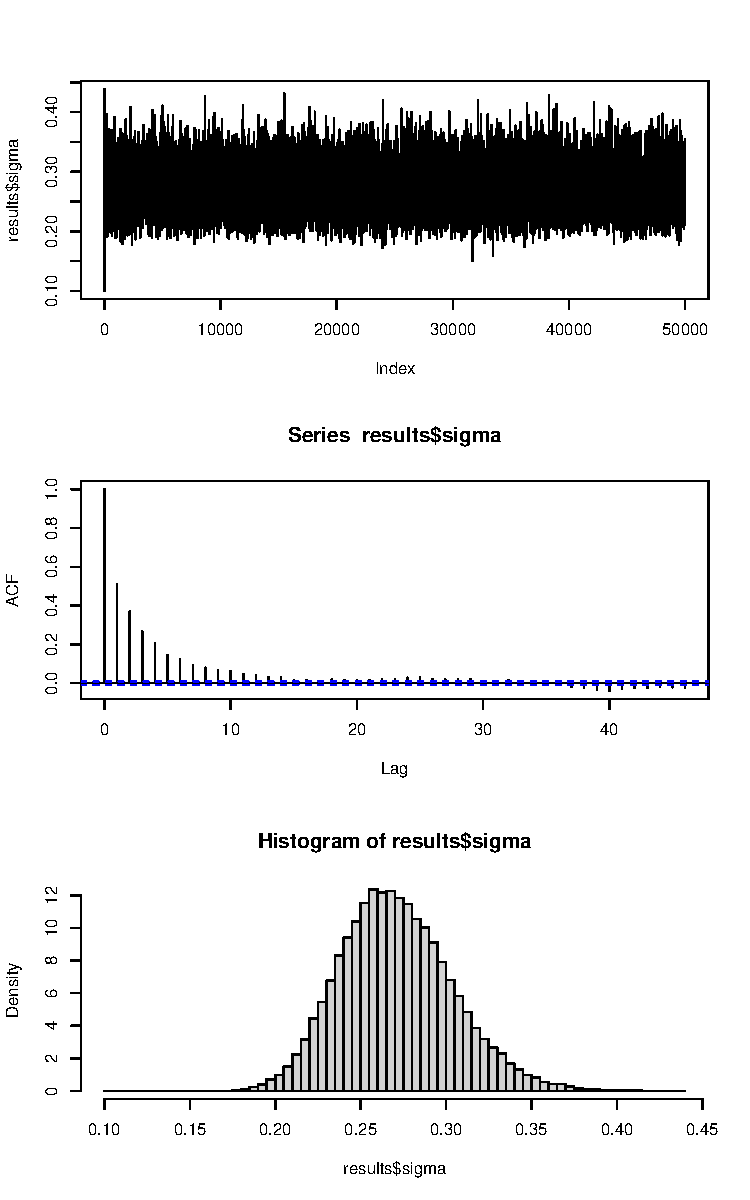
\includegraphics[width=0.8\linewidth]{Exercise-2-ny_files/figure-latex/1eSigmaRes-1} \end{center}

\begin{Shaded}
\begin{Highlighting}[]
\NormalTok{ylim }\OtherTok{=} \FunctionTok{c}\NormalTok{(}\FunctionTok{min}\NormalTok{(rain}\SpecialCharTok{$}\NormalTok{n.rain}\SpecialCharTok{/}\NormalTok{rain}\SpecialCharTok{$}\NormalTok{n.years), }\AttributeTok{max =} \FunctionTok{max}\NormalTok{(pSeq[}\DecValTok{1}\NormalTok{, ]))}
\FunctionTok{par}\NormalTok{(}\AttributeTok{mfrow =} \FunctionTok{c}\NormalTok{(}\DecValTok{1}\NormalTok{, }\DecValTok{1}\NormalTok{))}
\FunctionTok{plot}\NormalTok{(rain}\SpecialCharTok{$}\NormalTok{day, pSeq[}\DecValTok{1}\NormalTok{, ], }\AttributeTok{type =} \StringTok{"l"}\NormalTok{, }\AttributeTok{ylab =} \FunctionTok{expression}\NormalTok{(pi), }\AttributeTok{xlab =} \StringTok{"Day"}\NormalTok{, }\AttributeTok{ylim =}\NormalTok{ ylim,}
    \AttributeTok{col =} \StringTok{"gray"}\NormalTok{)}
\FunctionTok{lines}\NormalTok{(rain}\SpecialCharTok{$}\NormalTok{day, pSeq[N}\SpecialCharTok{/}\DecValTok{2}\NormalTok{, ], }\AttributeTok{type =} \StringTok{"l"}\NormalTok{, }\AttributeTok{ylim =}\NormalTok{ ylim, }\AttributeTok{col =} \StringTok{"cyan3"}\NormalTok{)}
\FunctionTok{lines}\NormalTok{(rain}\SpecialCharTok{$}\NormalTok{day, pSeq[N, ], }\AttributeTok{ylim =}\NormalTok{ ylim, }\AttributeTok{col =} \StringTok{"blue"}\NormalTok{, }\AttributeTok{lty =} \DecValTok{1}\NormalTok{)}
\FunctionTok{legend}\NormalTok{(}\AttributeTok{x =} \StringTok{"topright"}\NormalTok{, }\AttributeTok{legend =} \FunctionTok{c}\NormalTok{(}\StringTok{"Initial values"}\NormalTok{, }\StringTok{"Halfway"}\NormalTok{, }\StringTok{"Last iteration"}\NormalTok{),}
    \AttributeTok{lty =} \FunctionTok{c}\NormalTok{(}\DecValTok{1}\NormalTok{, }\DecValTok{1}\NormalTok{, }\DecValTok{1}\NormalTok{), }\AttributeTok{col =} \FunctionTok{c}\NormalTok{(}\StringTok{"gray"}\NormalTok{, }\StringTok{"cyan3"}\NormalTok{, }\StringTok{"blue"}\NormalTok{), }\AttributeTok{bg =} \StringTok{"transparent"}\NormalTok{)}
\end{Highlighting}
\end{Shaded}

\begin{figure}

{\centering 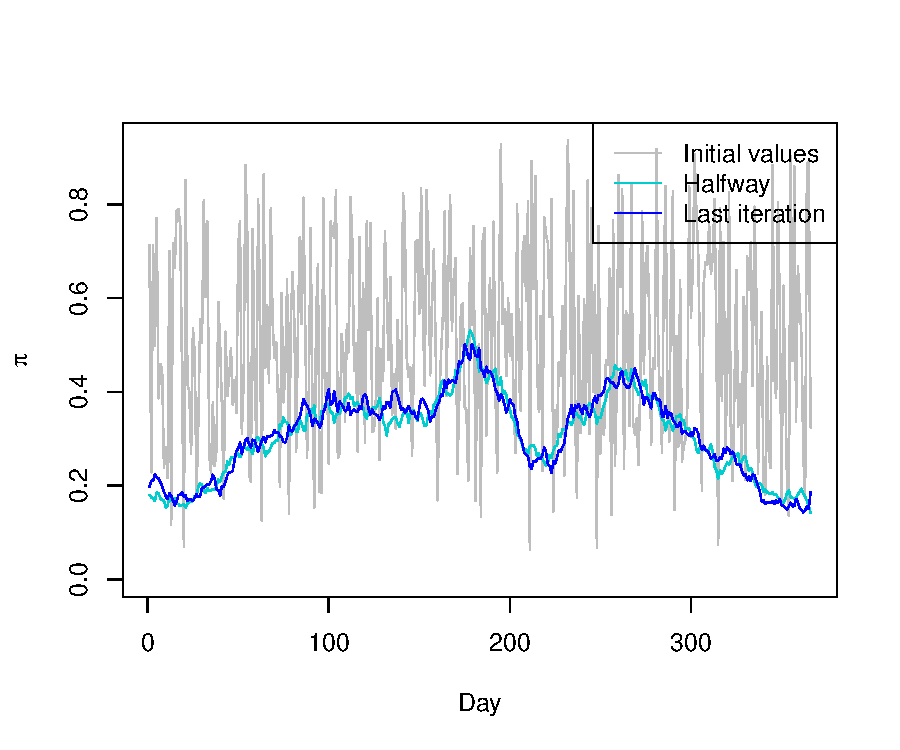
\includegraphics[width=0.8\linewidth]{Exercise-2-ny_files/figure-latex/1eEvolution-1} 

}

\caption{Make cap}\label{fig:1eEvolution}
\end{figure}

The initial values of \(\boldsymbol{\pi}\) show no resemblance to the Tokyo rainfall dataset probabilities in Figure \ref{fig:1eEvolution}

\begin{Shaded}
\begin{Highlighting}[]
\NormalTok{gg1e.df }\OtherTok{=} \FunctionTok{data.frame}\NormalTok{(}\AttributeTok{probPreds =}\NormalTok{ pSeq[N,], }\AttributeTok{l =}\NormalTok{ pSeqCI[}\DecValTok{2}\NormalTok{, ], }\AttributeTok{u =}\NormalTok{ pSeqCI[}\DecValTok{3}\NormalTok{,],}
                     \AttributeTok{meanPreds =}\NormalTok{ pSeqCI[}\DecValTok{1}\NormalTok{,], }\AttributeTok{probsReal =}\NormalTok{ n.rain}\SpecialCharTok{/}\NormalTok{n.years, }
                     \AttributeTok{day =}\NormalTok{ day)}
\FunctionTok{ggplot}\NormalTok{(}\AttributeTok{data =}\NormalTok{ gg1e.df, }\FunctionTok{aes}\NormalTok{(}\AttributeTok{x =}\NormalTok{ day, }\AttributeTok{y =}\NormalTok{ probPreds)) }\SpecialCharTok{+} 
  \CommentTok{\# geom\_ribbon(mapping = aes(ymin = l,ymax = u, fill = "CI"), alpha = 0.2) +}
  \FunctionTok{geom\_line}\NormalTok{(}\FunctionTok{aes}\NormalTok{(}\AttributeTok{color =} \StringTok{"tau"}\NormalTok{, }\AttributeTok{linetype=}\StringTok{"tau"}\NormalTok{)) }\SpecialCharTok{+}
  \FunctionTok{geom\_line}\NormalTok{(}\FunctionTok{aes}\NormalTok{(}\AttributeTok{y =}\NormalTok{ meanPreds, }\AttributeTok{color =} \StringTok{"mean"}\NormalTok{, }\AttributeTok{linetype=}\StringTok{"mean"}\NormalTok{)) }\SpecialCharTok{+}
  \FunctionTok{geom\_point}\NormalTok{(}\FunctionTok{aes}\NormalTok{(}\AttributeTok{y =}\NormalTok{ probsReal, }\AttributeTok{color =} \StringTok{"n.rain/n.years"}\NormalTok{,}
                \AttributeTok{size=}\StringTok{"n.rain/n.years"}\NormalTok{), }\AttributeTok{alpha =} \FloatTok{0.3}\NormalTok{) }\SpecialCharTok{+} 
  \FunctionTok{scale\_linetype\_manual}\NormalTok{(}
    \AttributeTok{name=}\StringTok{" "}\NormalTok{,}
    \AttributeTok{breaks =} \FunctionTok{c}\NormalTok{(}\StringTok{"tau"}\NormalTok{, }\StringTok{"mean"}\NormalTok{, }\StringTok{"n.rain/n.years"}\NormalTok{),}
    \AttributeTok{values =} \FunctionTok{c}\NormalTok{(}\DecValTok{2}\NormalTok{, }\DecValTok{1}\NormalTok{, }\ConstantTok{NA}\NormalTok{),}
    \AttributeTok{labels=}\FunctionTok{expression}\NormalTok{(pi}\SpecialCharTok{*}\NormalTok{(tau),}\StringTok{\textquotesingle{}Mean\textquotesingle{}}\NormalTok{,}\StringTok{\textquotesingle{}Data probability\textquotesingle{}}\NormalTok{)}
    \CommentTok{\# breaks = c("tau", "mean"),}
    \CommentTok{\# values = c(2, 1),}
    \CommentTok{\# labels=expression(pi*(tau),\textquotesingle{}Mean\textquotesingle{})}
    \CommentTok{\# values = c("tau"=1, "mean"=2, "n.rain/n.years"=2)}
\NormalTok{  ) }\SpecialCharTok{+}
  \FunctionTok{scale\_size\_manual}\NormalTok{(}
    \AttributeTok{name=}\StringTok{" "}\NormalTok{,}
    \AttributeTok{breaks =} \FunctionTok{c}\NormalTok{(}\StringTok{"tau"}\NormalTok{, }\StringTok{"mean"}\NormalTok{, }\StringTok{"n.rain/n.years"}\NormalTok{),}
    \AttributeTok{values =} \FunctionTok{c}\NormalTok{(}\ConstantTok{NA}\NormalTok{, }\ConstantTok{NA}\NormalTok{, }\FloatTok{0.1}\NormalTok{),}
    \AttributeTok{labels=}\FunctionTok{expression}\NormalTok{(pi}\SpecialCharTok{*}\NormalTok{(tau),}\StringTok{\textquotesingle{}Mean\textquotesingle{}}\NormalTok{,}\StringTok{\textquotesingle{}Data probability\textquotesingle{}}\NormalTok{)}
\NormalTok{    ) }\SpecialCharTok{+}
  \FunctionTok{scale\_color\_manual}\NormalTok{(}
    \AttributeTok{name=}\StringTok{" "}\NormalTok{,}
    \CommentTok{\# breaks = c("tau", "mean", "n.rain/n.years"),}
    \AttributeTok{values=}\FunctionTok{c}\NormalTok{(}\StringTok{"tau"}\OtherTok{=}\StringTok{"green"}\NormalTok{, }\StringTok{"mean"}\OtherTok{=}\StringTok{"black"}\NormalTok{,}\StringTok{"n.rain/n.years"}\OtherTok{=}\StringTok{"blue"}\NormalTok{),}
    \CommentTok{\# values=c("black", "green","pink"),}
    \AttributeTok{labels=}\FunctionTok{expression}\NormalTok{(pi}\SpecialCharTok{*}\NormalTok{(tau),}\StringTok{\textquotesingle{}Mean\textquotesingle{}}\NormalTok{,}\StringTok{\textquotesingle{}Data probability\textquotesingle{}}\NormalTok{)}
\NormalTok{  ) }\SpecialCharTok{+}
  \FunctionTok{labs}\NormalTok{(}\AttributeTok{y=}\StringTok{"Probabilities"}\NormalTok{, }\AttributeTok{x=}\StringTok{"Day"}\NormalTok{) }\SpecialCharTok{+}
  \FunctionTok{theme\_minimal}\NormalTok{()}
\end{Highlighting}
\end{Shaded}

\begin{figure}

{\centering 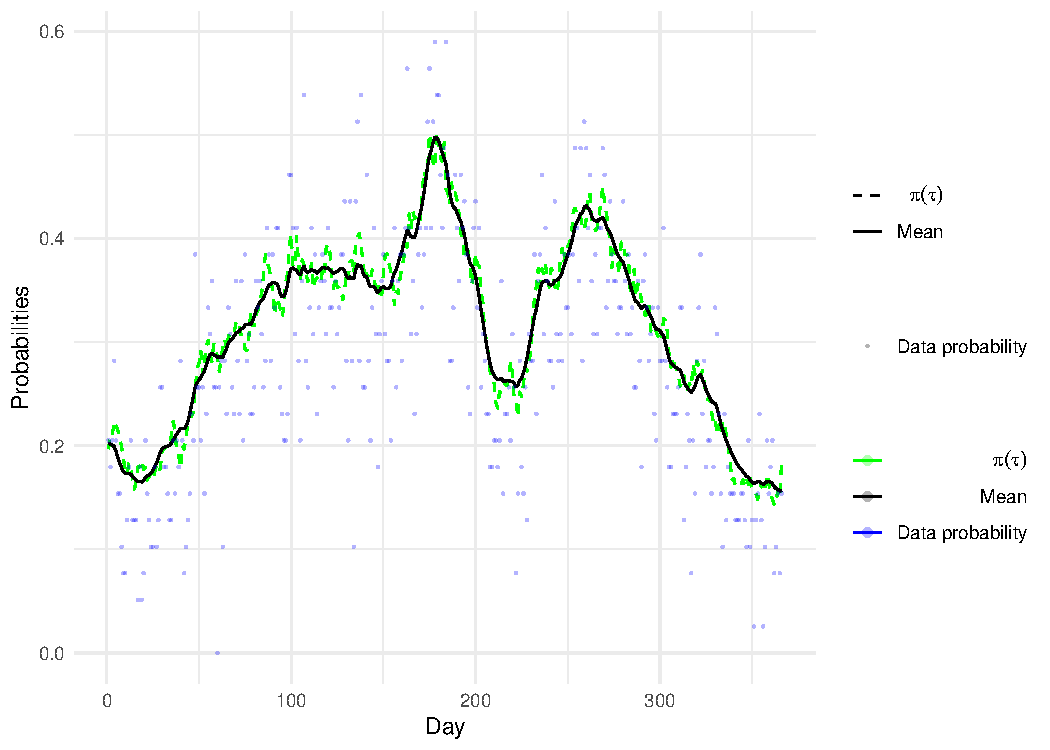
\includegraphics{Exercise-2-ny_files/figure-latex/1eggMean-1} 

}

\caption{The black line is the mean of all predicted probabilities $\pi$ excluding the burned predictions. The dashed green and blue lines are last iterations MCMC samples and the data probabilities, respectively.}\label{fig:1eggMean}
\end{figure}

\hypertarget{f-blocking-implementation}{%
\subsection{f) Blocking implementation}\label{f-blocking-implementation}}

Now we will go from sequentially updating \(\tau_t\) to perform block updates for each iteration. We will start by showing what mathematical implications that comes from blocking before we show the implementation and discuss the results. Rather than updating individual \(\tau_t\) parameters we will use a conditional prior proposal involving \(P( \boldsymbol{\tau}_{(a,b)}| \boldsymbol{\tau}_{-(a,b)})\), where \(\boldsymbol{\tau}_{(a,b)} = (\tau_a,...,\tau_b)\) for interval length \(M=b-a\). For intervals of length \(M>1\) we can simplify the acceptance probability as we did in section \ref{sec:1e}, only now

\begin{equation}\label{eq:1faccBlock}
  \frac{P(\boldsymbol{y}_\mathcal{I}| \boldsymbol{\tau}'_ \mathcal{I})}{P(\boldsymbol{y}_\mathcal{I}| \boldsymbol{\tau}_ \mathcal{I})}
  =
  \exp\left\{ \sum_{\mathcal{I}}y_i(\tau'_i - \tau_i) + n_i \ln \left( \frac{1+e^{\tau_i}}{1+e^{\tau'_i}} \right) \right\},
\end{equation}

where \(\mathcal{I}=(a,b)\). The conditional mean and precision used to draw the proposed values \(\boldsymbol{\tau}_ \mathcal{I}\) are given by
\[
\begin{aligned}
  &\boldsymbol{\mu}_{ \mathcal{I} \mid \mathcal{-I}} = \boldsymbol{\mu}_{\mathcal{I}} - \mathbf{Q}_{\mathcal{I}, \mathcal{I}}^{-1} \mathbf{Q}_{\mathcal{I},\mathcal{-I}} \left(\boldsymbol{\tau}_{\mathcal{-I}}-\boldsymbol{\mu}_{\mathcal{-I}}\right) 
  = -\mathbf{Q}_{\mathcal{I},\mathcal{I}}^{-1} \mathbf{Q}_{\mathcal{I},\mathcal{-I}}\boldsymbol{\tau}_{\mathcal{-I}}
  \\
  &\mathbf{Q}_{\mathcal{I} \mid \mathcal{-I}}=\mathbf{Q}_{\mathcal{I},\mathcal{I}}.
\end{aligned}
\]
Assuming \(1<M<T-2\), we get three different types of precision matrices which can be precomputated. Namely, one when the first day is included, the second where neither the first nor the last day is included, and the third where the last day is included in the set of days \(\mathcal{i}\). There are also only three different precision matrices for one iteration for the same day sets mentioned which also can be precomputated for each iteration. \textcolor{red}{precomputed or precomputated?}. The shape and size of said deflectors of the \(\mathbf{Q}\) matrix will not be discussed further, but can be computed from the \texttt{Qprecomp} function seen in the chunk below. The chunk also include the function for computing the acceptance ratio from Equation \eqref{eq:1faccBlock} and the implementation of the MCMC sampler.

\begin{Shaded}
\begin{Highlighting}[]
\NormalTok{acceptRatioBlock }\OtherTok{=} \ControlFlowTok{function}\NormalTok{(I, tauProp, tauPrev) \{}
    \FunctionTok{return}\NormalTok{(}\FunctionTok{exp}\NormalTok{(}\FunctionTok{sum}\NormalTok{(n.rain[I] }\SpecialCharTok{*}\NormalTok{ (tauProp }\SpecialCharTok{{-}}\NormalTok{ tauPrev)) }\SpecialCharTok{+} \FunctionTok{sum}\NormalTok{(rain}\SpecialCharTok{$}\NormalTok{n.years[I] }\SpecialCharTok{*}\NormalTok{ (}\FunctionTok{log}\NormalTok{(}\DecValTok{1} \SpecialCharTok{+}
        \FunctionTok{exp}\NormalTok{(tauPrev)) }\SpecialCharTok{{-}} \FunctionTok{log}\NormalTok{(}\DecValTok{1} \SpecialCharTok{+} \FunctionTok{exp}\NormalTok{(tauProp))))))}
\NormalTok{\}}

\NormalTok{Qprecomp }\OtherTok{=} \ControlFlowTok{function}\NormalTok{(M, }\AttributeTok{Ttot =} \DecValTok{366}\NormalTok{) \{}
    \DocumentationTok{\#\# Make intervals I}
\NormalTok{    n.sets }\OtherTok{=} \FunctionTok{ceiling}\NormalTok{(Ttot}\SpecialCharTok{/}\NormalTok{M)}
\NormalTok{    I }\OtherTok{=} \FunctionTok{matrix}\NormalTok{(}\DecValTok{1}\SpecialCharTok{:}\NormalTok{(M }\SpecialCharTok{*}\NormalTok{ (n.sets }\SpecialCharTok{{-}} \DecValTok{1}\NormalTok{)), }\AttributeTok{ncol =}\NormalTok{ n.sets }\SpecialCharTok{{-}} \DecValTok{1}\NormalTok{, }\AttributeTok{byrow =}\NormalTok{ F)}
\NormalTok{    Ires }\OtherTok{=}\NormalTok{ (I[M, n.sets }\SpecialCharTok{{-}} \DecValTok{1}\NormalTok{] }\SpecialCharTok{+} \DecValTok{1}\NormalTok{)}\SpecialCharTok{:}\NormalTok{Ttot}

    \CommentTok{\# Make Q}
\NormalTok{    Q }\OtherTok{=} \FunctionTok{triDiag}\NormalTok{(}\AttributeTok{diagonal =} \DecValTok{2}\NormalTok{, }\AttributeTok{upper =} \SpecialCharTok{{-}}\DecValTok{1}\NormalTok{, }\AttributeTok{lower =} \SpecialCharTok{{-}}\DecValTok{1}\NormalTok{, }\AttributeTok{nrow =}\NormalTok{ Ttot)}
\NormalTok{    Q[}\DecValTok{1}\NormalTok{, }\DecValTok{1}\NormalTok{] }\OtherTok{=} \DecValTok{1}
\NormalTok{    Q[Ttot, Ttot] }\OtherTok{=} \DecValTok{1}
    \CommentTok{\# Find the three Q\_AA}
\NormalTok{    Qaa1 }\OtherTok{=}\NormalTok{ Q[}\DecValTok{1}\SpecialCharTok{:}\NormalTok{M, }\DecValTok{1}\SpecialCharTok{:}\NormalTok{M]}
\NormalTok{    Qaa2 }\OtherTok{=}\NormalTok{ Q[}\DecValTok{2}\SpecialCharTok{:}\NormalTok{(M }\SpecialCharTok{+} \DecValTok{1}\NormalTok{), }\DecValTok{2}\SpecialCharTok{:}\NormalTok{(M }\SpecialCharTok{+} \DecValTok{1}\NormalTok{)]}
\NormalTok{    Qaa3 }\OtherTok{=}\NormalTok{ Q[Ires, Ires]}
\NormalTok{    Qaa1inv }\OtherTok{=} \FunctionTok{solve}\NormalTok{(Qaa1)}
\NormalTok{    Qaa2inv }\OtherTok{=} \FunctionTok{solve}\NormalTok{(Qaa2)}
\NormalTok{    Qaa3inv }\OtherTok{=} \FunctionTok{solve}\NormalTok{(Qaa3)}

\NormalTok{    Qmult }\OtherTok{=} \FunctionTok{list}\NormalTok{(}\AttributeTok{Qmult1 =} \SpecialCharTok{{-}}\NormalTok{Qaa1inv }\SpecialCharTok{\%*\%}\NormalTok{ Q[}\DecValTok{1}\SpecialCharTok{:}\NormalTok{M, }\SpecialCharTok{{-}}\NormalTok{(}\DecValTok{1}\SpecialCharTok{:}\NormalTok{M)])}
    \ControlFlowTok{for}\NormalTok{ (i }\ControlFlowTok{in} \DecValTok{2}\SpecialCharTok{:}\NormalTok{(n.sets }\SpecialCharTok{{-}} \DecValTok{1}\NormalTok{)) \{}
\NormalTok{        Qmult }\OtherTok{=} \FunctionTok{append}\NormalTok{(Qmult, }\FunctionTok{list}\NormalTok{(}\SpecialCharTok{{-}}\NormalTok{Qaa2inv }\SpecialCharTok{\%*\%}\NormalTok{ Q[I[, i], }\SpecialCharTok{{-}}\NormalTok{I[, i]]))}
\NormalTok{    \}}
\NormalTok{    Qmult }\OtherTok{=} \FunctionTok{append}\NormalTok{(Qmult, }\FunctionTok{list}\NormalTok{(}\SpecialCharTok{{-}}\NormalTok{Qaa3inv }\SpecialCharTok{\%*\%}\NormalTok{ Q[Ires, }\SpecialCharTok{{-}}\NormalTok{Ires]))}
    \FunctionTok{names}\NormalTok{(Qmult) }\OtherTok{=} \FunctionTok{sprintf}\NormalTok{(}\StringTok{"Qmult\%d"}\NormalTok{, }\DecValTok{1}\SpecialCharTok{:}\NormalTok{(n.sets))}

    \FunctionTok{return}\NormalTok{(}\FunctionTok{list}\NormalTok{(}\AttributeTok{Qaa1inv =}\NormalTok{ Qaa1inv, }\AttributeTok{Qaa2inv =}\NormalTok{ Qaa2inv, }\AttributeTok{Qaa3inv =}\NormalTok{ Qaa3inv, }\AttributeTok{Qmult =}\NormalTok{ Qmult,}
        \AttributeTok{n.sets =}\NormalTok{ n.sets, }\AttributeTok{I =}\NormalTok{ I, }\AttributeTok{Ires =}\NormalTok{ Ires))}
\NormalTok{\}}

\NormalTok{mcmcBlock }\OtherTok{=} \ControlFlowTok{function}\NormalTok{(N, }\AttributeTok{M =} \DecValTok{10}\NormalTok{, }\AttributeTok{sigma0 =} \FloatTok{0.1}\NormalTok{, }\AttributeTok{tau0 =} \FunctionTok{rnorm}\NormalTok{(}\DecValTok{366}\NormalTok{)) \{}
    \CommentTok{\# Allocate memory}
\NormalTok{    tau }\OtherTok{=} \FunctionTok{matrix}\NormalTok{(}\ConstantTok{NA}\NormalTok{, }\AttributeTok{nrow =}\NormalTok{ N, }\AttributeTok{ncol =}\NormalTok{ Ttot)  }\CommentTok{\# (N x T)}
\NormalTok{    sigma }\OtherTok{=} \FunctionTok{numeric}\NormalTok{(}\AttributeTok{length =}\NormalTok{ N)}
    \CommentTok{\# Assign initial values}
\NormalTok{    tau[}\DecValTok{1}\NormalTok{, ] }\OtherTok{=}\NormalTok{ tau0}
\NormalTok{    sigma[}\DecValTok{1}\NormalTok{] }\OtherTok{=}\NormalTok{ sigma0}
    \CommentTok{\# Assign Q matrices for easier access}
\NormalTok{    Qm }\OtherTok{=}\NormalTok{ Q}\SpecialCharTok{$}\NormalTok{Qmult  }\CommentTok{\# precomputed {-}QaaInverse * Qab}
\NormalTok{    n.sets }\OtherTok{=}\NormalTok{ Q}\SpecialCharTok{$}\NormalTok{n.sets}
\NormalTok{    Imat }\OtherTok{=}\NormalTok{ Q}\SpecialCharTok{$}\NormalTok{I  }\CommentTok{\# (M x (n.sets{-}1))}
\NormalTok{    Ires }\OtherTok{=}\NormalTok{ Q}\SpecialCharTok{$}\NormalTok{Ires}

    \CommentTok{\# Simulate N times}
\NormalTok{    accepted }\OtherTok{=} \DecValTok{0}
    \ControlFlowTok{for}\NormalTok{ (i }\ControlFlowTok{in} \DecValTok{2}\SpecialCharTok{:}\NormalTok{N) \{}
        \CommentTok{\# Perform first MH block step using upper left sub matrices of Q}
\NormalTok{        mhBlock }\OtherTok{=} \FunctionTok{mhBlockStep}\NormalTok{(tau[i }\SpecialCharTok{{-}} \DecValTok{1}\NormalTok{, ], Imat[, }\DecValTok{1}\NormalTok{], sigma[i }\SpecialCharTok{{-}} \DecValTok{1}\NormalTok{] }\SpecialCharTok{*}\NormalTok{ Q}\SpecialCharTok{$}\NormalTok{Qaa1inv,}
\NormalTok{            Qm}\SpecialCharTok{$}\NormalTok{Qmult1)}
\NormalTok{        tau[i, Imat[, }\DecValTok{1}\NormalTok{]] }\OtherTok{=}\NormalTok{ mhBlock}\SpecialCharTok{$}\NormalTok{tau}
\NormalTok{        accepted }\OtherTok{=}\NormalTok{ accepted }\SpecialCharTok{+}\NormalTok{ mhBlock}\SpecialCharTok{$}\NormalTok{accepted}

        \CommentTok{\# Precompute sigma\_u\^{}2 * Q\_AA\^{}{-}1 for all blocks where 1\textless{}t\textless{}366}
\NormalTok{        Sigma.mid }\OtherTok{=}\NormalTok{ sigma[i }\SpecialCharTok{{-}} \DecValTok{1}\NormalTok{] }\SpecialCharTok{*}\NormalTok{ Q}\SpecialCharTok{$}\NormalTok{Qaa2inv}
        \CommentTok{\# Perform MH block steps for days 1\textless{}t\textless{}366}
        \ControlFlowTok{for}\NormalTok{ (t }\ControlFlowTok{in} \DecValTok{2}\SpecialCharTok{:}\NormalTok{(n.sets }\SpecialCharTok{{-}} \DecValTok{1}\NormalTok{)) \{}
\NormalTok{            mhBlock }\OtherTok{=} \FunctionTok{mhBlockStep}\NormalTok{(tau[i }\SpecialCharTok{{-}} \DecValTok{1}\NormalTok{, ], Imat[, t], Sigma.mid, Qm[[t]])}
\NormalTok{            tau[i, Imat[, t]] }\OtherTok{=}\NormalTok{ mhBlock}\SpecialCharTok{$}\NormalTok{tau}
\NormalTok{            accepted }\OtherTok{=}\NormalTok{ accepted }\SpecialCharTok{+}\NormalTok{ mhBlock}\SpecialCharTok{$}\NormalTok{accepted}
\NormalTok{        \}}

        \CommentTok{\# Perform last MH block step using lower left sub matrices of Q}
\NormalTok{        mhBlock.last }\OtherTok{=} \FunctionTok{mhBlockStep}\NormalTok{(tau[i }\SpecialCharTok{{-}} \DecValTok{1}\NormalTok{, ], Ires, sigma[i }\SpecialCharTok{{-}} \DecValTok{1}\NormalTok{] }\SpecialCharTok{*}\NormalTok{ Q}\SpecialCharTok{$}\NormalTok{Qaa3inv,}
\NormalTok{            Qm[[n.sets]])}
\NormalTok{        tau[i, Ires] }\OtherTok{=}\NormalTok{ mhBlock.last}\SpecialCharTok{$}\NormalTok{tau}
\NormalTok{        accepted }\OtherTok{=}\NormalTok{ accepted }\SpecialCharTok{+}\NormalTok{ mhBlock.last}\SpecialCharTok{$}\NormalTok{accepted}

        \CommentTok{\# Perform Gibbs step for sigma\_u\^{}2}
\NormalTok{        tQt }\OtherTok{=} \FunctionTok{sum}\NormalTok{((}\FunctionTok{diff}\NormalTok{(tau[i, ]))}\SpecialCharTok{\^{}}\DecValTok{2}\NormalTok{)}
\NormalTok{        sigma[i] }\OtherTok{=} \DecValTok{1}\SpecialCharTok{/}\FunctionTok{rgamma}\NormalTok{(}\DecValTok{1}\NormalTok{, }\AttributeTok{shape =} \DecValTok{2} \SpecialCharTok{+}\NormalTok{ (Ttot }\SpecialCharTok{{-}} \DecValTok{1}\NormalTok{)}\SpecialCharTok{/}\DecValTok{2}\NormalTok{, }\AttributeTok{scale =} \FloatTok{0.05} \SpecialCharTok{+} \FloatTok{0.5} \SpecialCharTok{*}\NormalTok{ tQt)}

        \FunctionTok{setTxtProgressBar}\NormalTok{(pb, i)}
\NormalTok{    \}}
    \FunctionTok{close}\NormalTok{(pb)}
\NormalTok{    results }\OtherTok{=} \FunctionTok{list}\NormalTok{(tau, sigma, accepted}\SpecialCharTok{/}\NormalTok{(N }\SpecialCharTok{*}\NormalTok{ Ttot))}
    \FunctionTok{names}\NormalTok{(results) }\OtherTok{=} \FunctionTok{c}\NormalTok{(}\FunctionTok{paste0}\NormalTok{(}\StringTok{"tau"}\NormalTok{, M), }\FunctionTok{paste0}\NormalTok{(}\StringTok{"sigma"}\NormalTok{, M), }\FunctionTok{paste0}\NormalTok{(}\StringTok{"accProb"}\NormalTok{, M))}
    \FunctionTok{return}\NormalTok{(results)}
\NormalTok{\}}

\NormalTok{mhBlockStep }\OtherTok{=} \ControlFlowTok{function}\NormalTok{(tauPrev, I, Sigma, Qm.I) \{}
    \CommentTok{\# Inputs tauPrev : Previous sim tau values I : Indices for this block Sigma}
    \CommentTok{\# : sigma\_u\^{}2 * Q\_AA\^{}{-}1 Qm.I : {-}Q\_AA\^{}{-}1 x Q\_AB}

\NormalTok{    mu.ab }\OtherTok{=}\NormalTok{ Qm.I }\SpecialCharTok{\%*\%}\NormalTok{ tauPrev[}\SpecialCharTok{{-}}\NormalTok{I]}
\NormalTok{    tauProp }\OtherTok{=} \FunctionTok{mvrnorm}\NormalTok{(}\AttributeTok{n =} \DecValTok{1}\NormalTok{, }\AttributeTok{mu =}\NormalTok{ mu.ab, }\AttributeTok{Sigma =}\NormalTok{ Sigma)}
\NormalTok{    ratio }\OtherTok{=} \FunctionTok{acceptRatioBlock}\NormalTok{(I, tauProp, tauPrev[I])}
    \CommentTok{\# Random walk 1}
    \ControlFlowTok{if}\NormalTok{ (}\FunctionTok{runif}\NormalTok{(}\DecValTok{1}\NormalTok{) }\SpecialCharTok{\textless{}} \FunctionTok{min}\NormalTok{(}\FunctionTok{c}\NormalTok{(}\DecValTok{1}\NormalTok{, ratio))) \{}
        \FunctionTok{return}\NormalTok{(}\FunctionTok{list}\NormalTok{(}\AttributeTok{tau =}\NormalTok{ tauProp, }\AttributeTok{accepted =} \FunctionTok{length}\NormalTok{(I)))}
\NormalTok{    \} }\ControlFlowTok{else}\NormalTok{ \{}
        \FunctionTok{return}\NormalTok{(}\FunctionTok{list}\NormalTok{(}\AttributeTok{tau =}\NormalTok{ tauPrev[I], }\AttributeTok{accepted =} \DecValTok{0}\NormalTok{))}
\NormalTok{    \}}
\NormalTok{\}}

\NormalTok{M }\OtherTok{=} \DecValTok{10}
\NormalTok{N }\OtherTok{=} \DecValTok{5000}
\NormalTok{Ttot }\OtherTok{=} \DecValTok{366}
\end{Highlighting}
\end{Shaded}

In the following chunks we will run the block updating MCMC sampler for \(N=\) 5000 simulations with intervals of length \(M=\) 10. First we present the computation time followed by some visualizations for an overview of the results. Then we will discuss burning and do some computations and visualizations on the burned results.

\begin{Shaded}
\begin{Highlighting}[]

\NormalTok{Q }\OtherTok{=} \FunctionTok{Qprecomp}\NormalTok{(M)}
\NormalTok{pb }\OtherTok{=} \FunctionTok{txtProgressBar}\NormalTok{(}\AttributeTok{min =} \DecValTok{0}\NormalTok{, }\AttributeTok{max =}\NormalTok{ N, }\AttributeTok{initial =} \DecValTok{0}\NormalTok{)}
\FunctionTok{set.seed}\NormalTok{(}\DecValTok{321}\NormalTok{)}
\NormalTok{ptm }\OtherTok{=} \FunctionTok{proc.time}\NormalTok{()}
\CommentTok{\# profvis(\{results = mcmcBlock(N, rain, M)\}) \# For profiling}
\NormalTok{resultsBlock }\OtherTok{=} \FunctionTok{mcmcBlock}\NormalTok{(N, M)}
\end{Highlighting}
\end{Shaded}

\begin{verbatim}
## ================================================================================
\end{verbatim}

\begin{Shaded}
\begin{Highlighting}[]
\NormalTok{timeBlock }\OtherTok{=} \FunctionTok{proc.time}\NormalTok{() }\SpecialCharTok{{-}}\NormalTok{ ptm}
\NormalTok{timeBlock}
\end{Highlighting}
\end{Shaded}

\begin{verbatim}
##    user  system elapsed 
##   14.17    0.02   14.18
\end{verbatim}

\begin{Shaded}
\begin{Highlighting}[]
\NormalTok{pSeq }\OtherTok{=} \FunctionTok{apply}\NormalTok{(resultsBlock}\SpecialCharTok{$}\NormalTok{tau, }\DecValTok{2}\NormalTok{, link)}
\FunctionTok{par}\NormalTok{(}\AttributeTok{mfrow =} \FunctionTok{c}\NormalTok{(}\DecValTok{3}\NormalTok{, }\DecValTok{3}\NormalTok{))}
\FunctionTok{plotTAH}\NormalTok{(pSeq[, }\DecValTok{1}\NormalTok{], }\AttributeTok{burn =} \DecValTok{2000}\NormalTok{)}
\FunctionTok{plotTAH}\NormalTok{(pSeq[, }\DecValTok{201}\NormalTok{], }\AttributeTok{burn =} \DecValTok{2000}\NormalTok{)}
\FunctionTok{plotTAH}\NormalTok{(pSeq[, }\DecValTok{366}\NormalTok{], }\AttributeTok{burn =} \DecValTok{2000}\NormalTok{)}
\end{Highlighting}
\end{Shaded}

\begin{center}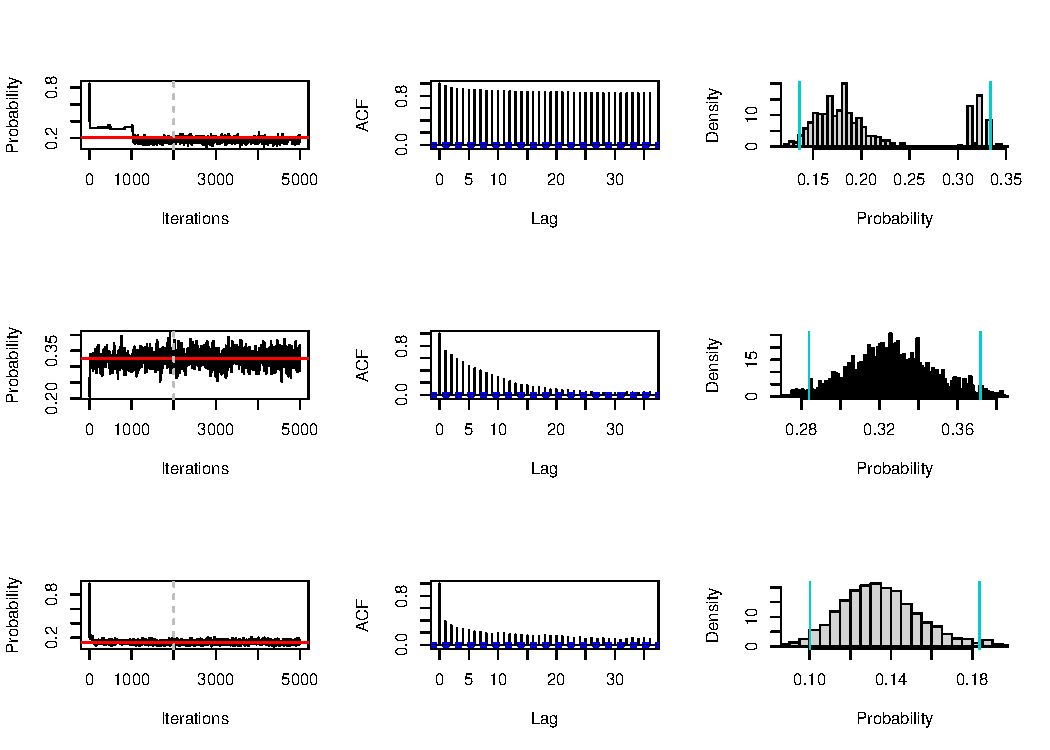
\includegraphics{Exercise-2-ny_files/figure-latex/1fcomputations, options-1} \end{center}

\begin{Shaded}
\begin{Highlighting}[]
\NormalTok{pSeqCI }\OtherTok{=} \FunctionTok{apply}\NormalTok{(pSeq, }\DecValTok{2}\NormalTok{, CImean)  }\CommentTok{\# Compute mean and credibility interval}

\CommentTok{\# Burn}
\NormalTok{burn }\OtherTok{=} \DecValTok{2000}
\NormalTok{resultsB }\OtherTok{=}\NormalTok{ resultsBlock}
\NormalTok{resultsB}\SpecialCharTok{$}\NormalTok{tau }\OtherTok{=}\NormalTok{ resultsBlock}\SpecialCharTok{$}\NormalTok{tau[burn}\SpecialCharTok{:}\NormalTok{N, ]}
\NormalTok{resultsB}\SpecialCharTok{$}\NormalTok{sigma }\OtherTok{=}\NormalTok{ resultsBlock}\SpecialCharTok{$}\NormalTok{sigma[burn}\SpecialCharTok{:}\NormalTok{N]}
\NormalTok{pSeqB }\OtherTok{=}\NormalTok{ pSeq[burn}\SpecialCharTok{:}\NormalTok{N, ]}
\NormalTok{pSeqCIB }\OtherTok{=} \FunctionTok{apply}\NormalTok{(pSeqB, }\DecValTok{2}\NormalTok{, CImean)  }\CommentTok{\# Compute mean and credibility interval}
\NormalTok{ciAndMean }\OtherTok{=} \FunctionTok{rbind}\NormalTok{((pSeqCI[, }\DecValTok{1}\NormalTok{]), (pSeqCIB[, }\DecValTok{1}\NormalTok{]), (pSeqCI[, }\DecValTok{201}\NormalTok{]), (pSeqCIB[, }\DecValTok{201}\NormalTok{]),}
\NormalTok{    (pSeqCI[, }\DecValTok{366}\NormalTok{]), (pSeqCIB[, }\DecValTok{366}\NormalTok{]), }\FunctionTok{CImean}\NormalTok{(resultsBlock}\SpecialCharTok{$}\NormalTok{sigma), }\FunctionTok{CImean}\NormalTok{(resultsB}\SpecialCharTok{$}\NormalTok{sigma))}
\FunctionTok{rownames}\NormalTok{(ciAndMean) }\OtherTok{=} \FunctionTok{c}\NormalTok{(}\StringTok{"1"}\NormalTok{, }\StringTok{"1 B"}\NormalTok{, }\StringTok{"201"}\NormalTok{, }\StringTok{"201 B"}\NormalTok{, }\StringTok{"366"}\NormalTok{, }\StringTok{"366 B"}\NormalTok{, }\StringTok{"sigma"}\NormalTok{, }\StringTok{"sigma B"}\NormalTok{)}
\CommentTok{\# knitr::kable(round(ciAndMean,4), caption = \textquotesingle{}mean and stuff\textquotesingle{})}
\NormalTok{knitr}\SpecialCharTok{::}\FunctionTok{kable}\NormalTok{(}\FunctionTok{round}\NormalTok{(ciAndMean, }\DecValTok{4}\NormalTok{), }\AttributeTok{caption =} \StringTok{"mean and stuff"}\NormalTok{)}
\end{Highlighting}
\end{Shaded}

\begin{table}

\caption{\label{tab:1fburn}mean and stuff}
\centering
\begin{tabular}[t]{l|r|r|r}
\hline
  & mean & 2.5\% & 97.5\%\\
\hline
1 & 0.2061 & 0.1358 & 0.3337\\
\hline
1 B & 0.1770 & 0.1350 & 0.2260\\
\hline
201 & 0.3259 & 0.2839 & 0.3717\\
\hline
201 B & 0.3276 & 0.2832 & 0.3718\\
\hline
366 & 0.1354 & 0.1002 & 0.1836\\
\hline
366 B & 0.1339 & 0.0988 & 0.1763\\
\hline
sigma & 0.0044 & 0.0021 & 0.0061\\
\hline
sigma B & 0.0051 & 0.0041 & 0.0062\\
\hline
\end{tabular}
\end{table}

\begin{Shaded}
\begin{Highlighting}[]
\FunctionTok{par}\NormalTok{(}\AttributeTok{mfrow =} \FunctionTok{c}\NormalTok{(}\DecValTok{3}\NormalTok{, }\DecValTok{3}\NormalTok{))}
\FunctionTok{plotTAH}\NormalTok{(pSeqB[, }\DecValTok{1}\NormalTok{], }\AttributeTok{burn =} \DecValTok{2000}\NormalTok{)}
\FunctionTok{plotTAH}\NormalTok{(pSeqB[, }\DecValTok{201}\NormalTok{], }\AttributeTok{burn =} \DecValTok{2000}\NormalTok{)}
\FunctionTok{plotTAH}\NormalTok{(pSeqB[, }\DecValTok{366}\NormalTok{], }\AttributeTok{burn =} \DecValTok{2000}\NormalTok{)}
\end{Highlighting}
\end{Shaded}

\begin{center}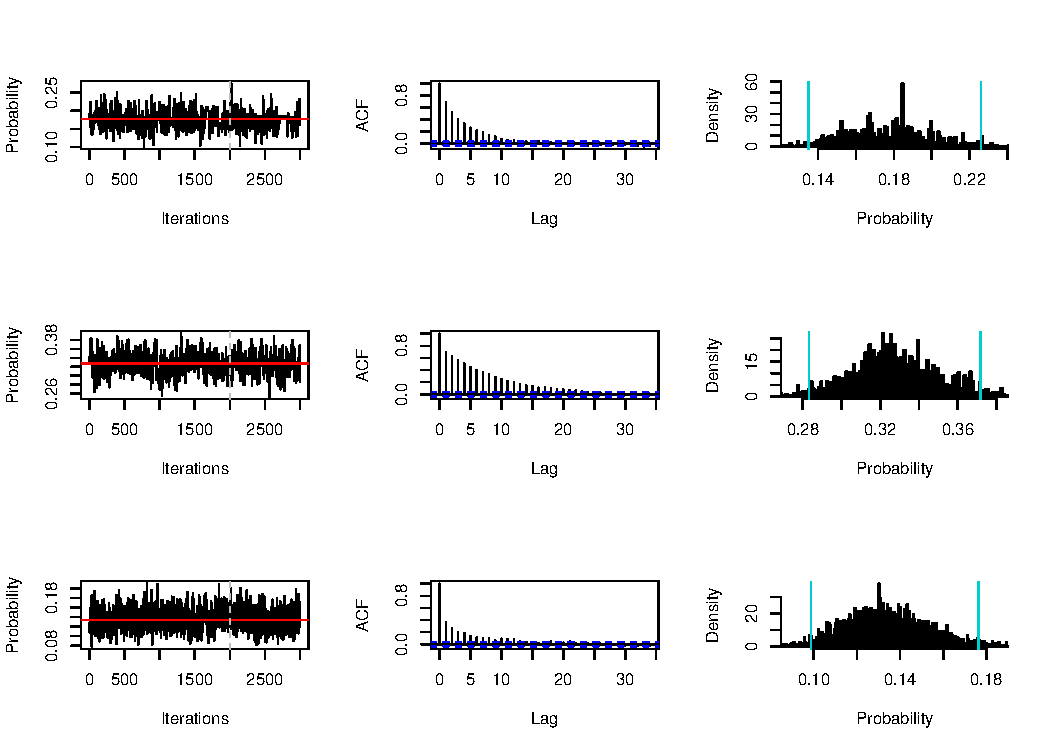
\includegraphics{Exercise-2-ny_files/figure-latex/1fplotBurn, options-1} \end{center}

\begin{Shaded}
\begin{Highlighting}[]
\NormalTok{gg1e.df }\OtherTok{=} \FunctionTok{data.frame}\NormalTok{(}\AttributeTok{probPreds =}\NormalTok{ pSeq[N, ], }\AttributeTok{l =}\NormalTok{ pSeqCI[}\DecValTok{2}\NormalTok{, ], }\AttributeTok{u =}\NormalTok{ pSeqCI[}\DecValTok{3}\NormalTok{, ], }\AttributeTok{meanPreds =}\NormalTok{ pSeqCI[}\DecValTok{1}\NormalTok{,}
\NormalTok{    ], }\AttributeTok{probsReal =}\NormalTok{ n.rain}\SpecialCharTok{/}\NormalTok{n.years, }\AttributeTok{day =}\NormalTok{ day)}
\FunctionTok{ggplot}\NormalTok{(}\AttributeTok{data =}\NormalTok{ gg1e.df, }\FunctionTok{aes}\NormalTok{(}\AttributeTok{x =}\NormalTok{ day, }\AttributeTok{y =}\NormalTok{ probPreds)) }\SpecialCharTok{+} \FunctionTok{geom\_line}\NormalTok{(}\FunctionTok{aes}\NormalTok{(}\AttributeTok{color =} \StringTok{"tau"}\NormalTok{,}
    \AttributeTok{linetype =} \StringTok{"tau"}\NormalTok{)) }\SpecialCharTok{+} \FunctionTok{geom\_line}\NormalTok{(}\FunctionTok{aes}\NormalTok{(}\AttributeTok{y =}\NormalTok{ meanPreds, }\AttributeTok{color =} \StringTok{"mean"}\NormalTok{, }\AttributeTok{linetype =} \StringTok{"mean"}\NormalTok{)) }\SpecialCharTok{+}
    \FunctionTok{geom\_point}\NormalTok{(}\FunctionTok{aes}\NormalTok{(}\AttributeTok{y =}\NormalTok{ probsReal, }\AttributeTok{color =} \StringTok{"n.rain/n.years"}\NormalTok{, }\AttributeTok{size =} \StringTok{"n.rain/n.years"}\NormalTok{),}
        \AttributeTok{alpha =} \FloatTok{0.3}\NormalTok{) }\SpecialCharTok{+} \FunctionTok{scale\_linetype\_manual}\NormalTok{(}\AttributeTok{name =} \StringTok{" "}\NormalTok{, }\AttributeTok{breaks =} \FunctionTok{c}\NormalTok{(}\StringTok{"tau"}\NormalTok{, }\StringTok{"mean"}\NormalTok{,}
    \StringTok{"n.rain/n.years"}\NormalTok{), }\AttributeTok{values =} \FunctionTok{c}\NormalTok{(}\DecValTok{2}\NormalTok{, }\DecValTok{1}\NormalTok{, }\ConstantTok{NA}\NormalTok{), }\AttributeTok{labels =} \FunctionTok{expression}\NormalTok{(pi }\SpecialCharTok{*}\NormalTok{ (tau), }\StringTok{"Mean"}\NormalTok{,}
    \StringTok{"Data probability"}\NormalTok{)) }\SpecialCharTok{+} \FunctionTok{scale\_size\_manual}\NormalTok{(}\AttributeTok{name =} \StringTok{" "}\NormalTok{, }\AttributeTok{breaks =} \FunctionTok{c}\NormalTok{(}\StringTok{"tau"}\NormalTok{, }\StringTok{"mean"}\NormalTok{,}
    \StringTok{"n.rain/n.years"}\NormalTok{), }\AttributeTok{values =} \FunctionTok{c}\NormalTok{(}\ConstantTok{NA}\NormalTok{, }\ConstantTok{NA}\NormalTok{, }\FloatTok{0.1}\NormalTok{), }\AttributeTok{labels =} \FunctionTok{expression}\NormalTok{(pi }\SpecialCharTok{*}\NormalTok{ (tau), }\StringTok{"Mean"}\NormalTok{,}
    \StringTok{"Data probability"}\NormalTok{)) }\SpecialCharTok{+} \FunctionTok{scale\_color\_manual}\NormalTok{(}\AttributeTok{name =} \StringTok{" "}\NormalTok{, }\AttributeTok{values =} \FunctionTok{c}\NormalTok{(}\AttributeTok{tau =} \StringTok{"green"}\NormalTok{,}
    \AttributeTok{mean =} \StringTok{"black"}\NormalTok{, }\StringTok{\textasciigrave{}}\AttributeTok{n.rain/n.years}\StringTok{\textasciigrave{}} \OtherTok{=} \StringTok{"blue"}\NormalTok{), }\AttributeTok{labels =} \FunctionTok{expression}\NormalTok{(pi }\SpecialCharTok{*}\NormalTok{ (tau), }\StringTok{"Mean"}\NormalTok{,}
    \StringTok{"Data probability"}\NormalTok{)) }\SpecialCharTok{+} \FunctionTok{labs}\NormalTok{(}\AttributeTok{y =} \StringTok{"Probabilities"}\NormalTok{, }\AttributeTok{x =} \StringTok{"Day"}\NormalTok{) }\SpecialCharTok{+} \FunctionTok{theme\_minimal}\NormalTok{()}
\end{Highlighting}
\end{Shaded}

\begin{figure}

{\centering 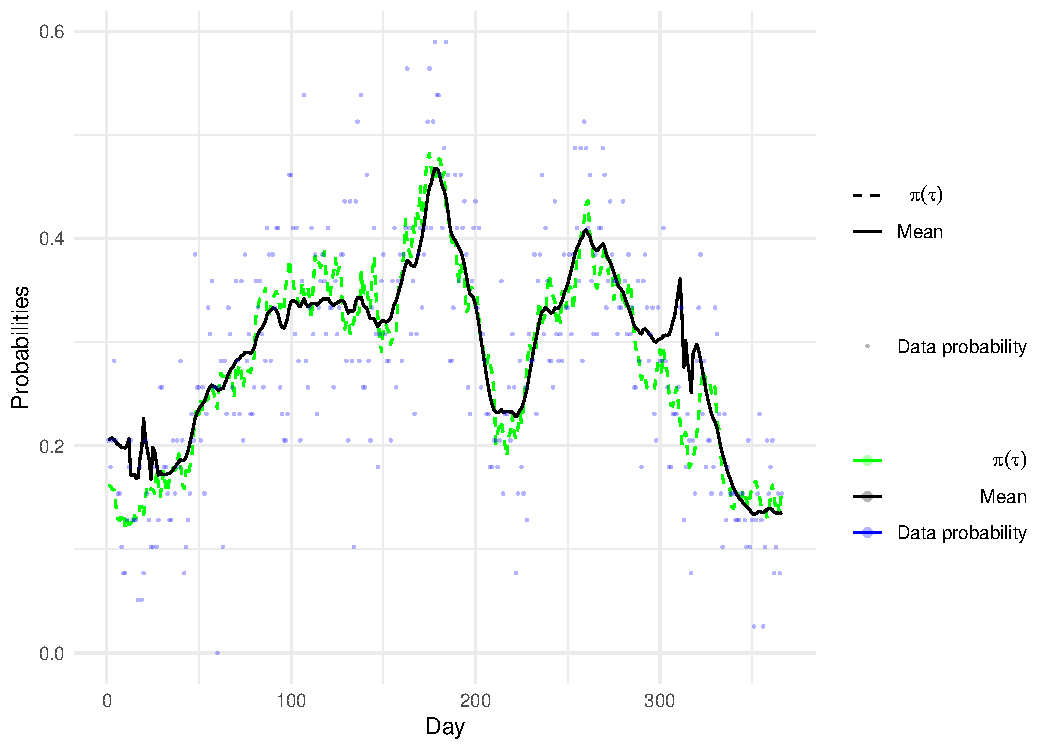
\includegraphics{Exercise-2-ny_files/figure-latex/1fggMean-1} 

}

\caption{makeCap}\label{fig:1fggMean}
\end{figure}

\begin{Shaded}
\begin{Highlighting}[]
\NormalTok{N }\OtherTok{=} \DecValTok{5000}

\NormalTok{Mlist }\OtherTok{=} \FunctionTok{c}\NormalTok{(}\DecValTok{2}\NormalTok{, }\DecValTok{5}\NormalTok{, }\DecValTok{10}\NormalTok{, }\DecValTok{15}\NormalTok{, }\DecValTok{20}\NormalTok{, }\DecValTok{25}\NormalTok{, }\DecValTok{40}\NormalTok{, }\DecValTok{80}\NormalTok{)}
\NormalTok{n.runs }\OtherTok{=} \FunctionTok{length}\NormalTok{(Mlist)}
\NormalTok{resultList }\OtherTok{=} \FunctionTok{list}\NormalTok{()}
\NormalTok{time }\OtherTok{=} \FunctionTok{c}\NormalTok{()}
\FunctionTok{set.seed}\NormalTok{(}\DecValTok{321}\NormalTok{)}
\NormalTok{tau0 }\OtherTok{=} \FunctionTok{rnorm}\NormalTok{(}\DecValTok{366}\NormalTok{)}

\ControlFlowTok{for}\NormalTok{ (i }\ControlFlowTok{in} \DecValTok{1}\SpecialCharTok{:}\FunctionTok{length}\NormalTok{(Mlist)) \{}
    \FunctionTok{set.seed}\NormalTok{(}\DecValTok{321}\NormalTok{)}
\NormalTok{    pb }\OtherTok{=} \FunctionTok{txtProgressBar}\NormalTok{(}\AttributeTok{min =} \DecValTok{0}\NormalTok{, }\AttributeTok{max =}\NormalTok{ N, }\AttributeTok{initial =} \DecValTok{0}\NormalTok{)}
\NormalTok{    Q }\OtherTok{=} \FunctionTok{Qprecomp}\NormalTok{(Mlist[i], Ttot)}
\NormalTok{    start }\OtherTok{=} \FunctionTok{proc.time}\NormalTok{()[}\DecValTok{3}\NormalTok{]}
\NormalTok{    resultList }\OtherTok{=} \FunctionTok{append}\NormalTok{(resultList, }\FunctionTok{mcmcBlock}\NormalTok{(N, Mlist[i], }\AttributeTok{tau0 =}\NormalTok{ tau0))}
\NormalTok{    time }\OtherTok{=} \FunctionTok{c}\NormalTok{(time, }\FunctionTok{proc.time}\NormalTok{()[}\DecValTok{3}\NormalTok{] }\SpecialCharTok{{-}}\NormalTok{ start)}
\NormalTok{\}}
\end{Highlighting}
\end{Shaded}

\begin{verbatim}
## ================================================================================
## ================================================================================
## ================================================================================
## ================================================================================
## ================================================================================
## ================================================================================
## ================================================================================
## ================================================================================
\end{verbatim}

The chunk above ran the MCMC sampler for \(N=\) 5000 with interval lengths \(\boldsymbol{M}=\{ 2, 5, 10, 15, 20, 25, 40, 80 \}\). In Figure \ref{fig:1fTuneTimeAcc} produced by the chunk below we see that the acceptance probability decrease with increasing interval lengths \(M\). For a RW(1) model, a rule of thumb is to have acceptance probability \(\alpha \in (0.2,0.5)\) which coincide with the acceptance probability for \(M=20\). We also notice that the computation time decrease for interval lengths \(M \leq 20\) before it starts to increase. Thus, based on these results, \(M=20\) seems like a good candidate for interval length.

\begin{Shaded}
\begin{Highlighting}[]
\NormalTok{accProbsBlock }\OtherTok{=} \FunctionTok{c}\NormalTok{()}
\ControlFlowTok{for}\NormalTok{ (m }\ControlFlowTok{in}\NormalTok{ Mlist) \{}
\NormalTok{    accProbsBlock }\OtherTok{=} \FunctionTok{c}\NormalTok{(accProbsBlock, resultList[[}\FunctionTok{paste0}\NormalTok{(}\StringTok{"accProb"}\NormalTok{, m)]])}
\NormalTok{\}}
\FunctionTok{par}\NormalTok{(}\AttributeTok{mfrow =} \FunctionTok{c}\NormalTok{(}\DecValTok{1}\NormalTok{, }\DecValTok{1}\NormalTok{))}
\FunctionTok{plot}\NormalTok{(Mlist, time, }\AttributeTok{ylim =} \FunctionTok{c}\NormalTok{(}\DecValTok{0}\NormalTok{, }\FunctionTok{max}\NormalTok{(}\FunctionTok{c}\NormalTok{(time, }\DecValTok{100} \SpecialCharTok{*}\NormalTok{ accProbsBlock))), }\AttributeTok{pch =} \DecValTok{16}\NormalTok{, }\AttributeTok{xaxt =} \StringTok{"n"}\NormalTok{,}
    \AttributeTok{xlab =} \StringTok{"M"}\NormalTok{, }\AttributeTok{ylab =} \StringTok{"Time/acceptance probability (\%)"}\NormalTok{)}
\FunctionTok{points}\NormalTok{(Mlist, accProbsBlock }\SpecialCharTok{*} \DecValTok{100}\NormalTok{, }\AttributeTok{col =} \StringTok{"cyan3"}\NormalTok{, }\AttributeTok{pch =} \DecValTok{16}\NormalTok{)}
\FunctionTok{abline}\NormalTok{(}\AttributeTok{h =} \FunctionTok{c}\NormalTok{(}\DecValTok{20}\NormalTok{, }\DecValTok{50}\NormalTok{), }\AttributeTok{lty =} \DecValTok{2}\NormalTok{)}
\FunctionTok{axis}\NormalTok{(}\DecValTok{1}\NormalTok{, }\AttributeTok{at =}\NormalTok{ Mlist)}
\end{Highlighting}
\end{Shaded}

\begin{figure}

{\centering \includegraphics[width=0.8\linewidth]{Exercise-2-ny_files/figure-latex/1fTuneTimeAcc-1} 

}

\caption{Computation time for different values of $M$ along with the respective acceptance probability. Dashed horizontal lines show desired acceptance probability for RW(1).}\label{fig:1fTuneTimeAcc}
\end{figure}

To further investigate candidates for interval lengths we consider the traceplots in Figure \ref{fig:1fTraceBlockInit} produced by the chunk below. Since all fits were run for only \$N= 5000 \$ iterations, it is difficult to say whether the chain has fully converged. The three plot rows in the bottom show clear signs of not convergence. Still, the resulting traceplots does not rule out our favorable candidate from before, namely \(M=20\), showing promising convergence rate.

\begin{Shaded}
\begin{Highlighting}[]
\NormalTok{dToPlot }\OtherTok{=} \FunctionTok{c}\NormalTok{(}\DecValTok{1}\NormalTok{, }\DecValTok{201}\NormalTok{, }\DecValTok{366}\NormalTok{)}
\FunctionTok{par}\NormalTok{(}\AttributeTok{mfrow =} \FunctionTok{c}\NormalTok{(}\FunctionTok{length}\NormalTok{(Mlist), }\FunctionTok{length}\NormalTok{(dToPlot)), }\AttributeTok{mar =} \FunctionTok{c}\NormalTok{(}\DecValTok{2}\NormalTok{, }\DecValTok{2}\NormalTok{, }\FloatTok{0.1}\NormalTok{, }\DecValTok{1}\NormalTok{))}
\ControlFlowTok{for}\NormalTok{ (i }\ControlFlowTok{in} \DecValTok{1}\SpecialCharTok{:}\FunctionTok{length}\NormalTok{(Mlist)) \{}
\NormalTok{    xaxt }\OtherTok{=} \FunctionTok{ifelse}\NormalTok{(i }\SpecialCharTok{==} \FunctionTok{length}\NormalTok{(Mlist), }\StringTok{"s"}\NormalTok{, }\StringTok{"n"}\NormalTok{)}
    \ControlFlowTok{for}\NormalTok{ (t }\ControlFlowTok{in}\NormalTok{ dToPlot) \{}
        \FunctionTok{plot}\NormalTok{(resultList[[}\FunctionTok{paste0}\NormalTok{(}\StringTok{"tau"}\NormalTok{, Mlist[i])]][, t], }\AttributeTok{type =} \StringTok{"l"}\NormalTok{, }\AttributeTok{xlab =} \StringTok{""}\NormalTok{, }\AttributeTok{ylab =} \StringTok{""}\NormalTok{,}
            \AttributeTok{xaxt =}\NormalTok{ xaxt)}
\NormalTok{    \}}
\NormalTok{\}}
\end{Highlighting}
\end{Shaded}

\begin{figure}

{\centering \includegraphics[width=0.8\linewidth]{Exercise-2-ny_files/figure-latex/1fTraceBlockInit-1} 

}

\caption{Trace plots of $\boldsymbol{\pi}$ for low to high value of the tuning param $M$ from top to bottom, respectively, for different days $t$.}\label{fig:1fTraceBlockInit}
\end{figure}

So, some values of \(M\) show promicing results, but we still need to compare them to the real data. Since all traceplots in Figure \ref{fig:1fTraceBlockInit} show signs of not convergence for early iterations we chose to burn some values. The amount burned is shown in the chunk below.

\begin{Shaded}
\begin{Highlighting}[]
\NormalTok{burnTune }\OtherTok{=} \DecValTok{1000}  \CommentTok{\# burn amount for M tuning}
\NormalTok{pMeanBlockMat }\OtherTok{=} \FunctionTok{matrix}\NormalTok{(}\ConstantTok{NA}\NormalTok{, }\AttributeTok{nrow =} \FunctionTok{length}\NormalTok{(Mlist), }\AttributeTok{ncol =}\NormalTok{ Ttot)}
\ControlFlowTok{for}\NormalTok{ (i }\ControlFlowTok{in} \DecValTok{1}\SpecialCharTok{:}\FunctionTok{length}\NormalTok{(Mlist)) \{}
\NormalTok{    pMeanBlockMat[i, ] }\OtherTok{=} \FunctionTok{apply}\NormalTok{(}\FunctionTok{link}\NormalTok{(resultList[[}\FunctionTok{paste0}\NormalTok{(}\StringTok{"tau"}\NormalTok{, Mlist[i])]][burnTune}\SpecialCharTok{:}\NormalTok{N,}
\NormalTok{        ]), }\DecValTok{2}\NormalTok{, mean)}
\NormalTok{\}}
\NormalTok{a }\OtherTok{=} \DecValTok{0}
\end{Highlighting}
\end{Shaded}

M = 25 shows good results

\begin{Shaded}
\begin{Highlighting}[]
\NormalTok{colfunc }\OtherTok{\textless{}{-}} \FunctionTok{colorRampPalette}\NormalTok{(}\FunctionTok{c}\NormalTok{(}\StringTok{"red"}\NormalTok{, }\StringTok{"yellow"}\NormalTok{, }\StringTok{"springgreen"}\NormalTok{, }\StringTok{"royalblue"}\NormalTok{))}
\NormalTok{c }\OtherTok{=} \FunctionTok{colfunc}\NormalTok{(}\FunctionTok{length}\NormalTok{(pMeanBlockMat[, }\DecValTok{1}\NormalTok{]))}
\NormalTok{diffTune }\OtherTok{=} \FunctionTok{numeric}\NormalTok{()}
\NormalTok{pReal }\OtherTok{=}\NormalTok{ n.rain}\SpecialCharTok{/}\NormalTok{n.years}
\CommentTok{\# plot(day,pReal, pch=4, cex=0.5)}
\FunctionTok{par}\NormalTok{(}\AttributeTok{mfrow =} \FunctionTok{c}\NormalTok{(}\FunctionTok{ceiling}\NormalTok{(}\FunctionTok{length}\NormalTok{(Mlist)}\SpecialCharTok{/}\DecValTok{2}\NormalTok{), }\DecValTok{2}\NormalTok{), }\AttributeTok{mar =} \FunctionTok{c}\NormalTok{(}\DecValTok{1}\NormalTok{, }\DecValTok{2}\NormalTok{, }\DecValTok{1}\NormalTok{, }\DecValTok{1}\NormalTok{))}
\ControlFlowTok{for}\NormalTok{ (i }\ControlFlowTok{in} \DecValTok{1}\SpecialCharTok{:}\FunctionTok{length}\NormalTok{(pMeanBlockMat[, }\DecValTok{1}\NormalTok{])) \{}
    \FunctionTok{ifelse}\NormalTok{(i }\SpecialCharTok{\textless{}} \FunctionTok{length}\NormalTok{(pMeanBlockMat[, }\DecValTok{1}\NormalTok{]) }\SpecialCharTok{{-}} \DecValTok{1}\NormalTok{, }\ConstantTok{NA}\NormalTok{, }\FunctionTok{par}\NormalTok{(}\AttributeTok{mar =} \FunctionTok{c}\NormalTok{(}\DecValTok{2}\NormalTok{, }\DecValTok{2}\NormalTok{, }\DecValTok{1}\NormalTok{, }\DecValTok{1}\NormalTok{)))}
\NormalTok{    yaxt }\OtherTok{=} \FunctionTok{ifelse}\NormalTok{(i}\SpecialCharTok{\%\%}\DecValTok{2}\NormalTok{, }\StringTok{"s"}\NormalTok{, }\StringTok{"n"}\NormalTok{)}
\NormalTok{    xaxt }\OtherTok{=} \FunctionTok{ifelse}\NormalTok{(i }\SpecialCharTok{\textless{}} \FunctionTok{length}\NormalTok{(pMeanBlockMat[, }\DecValTok{1}\NormalTok{]) }\SpecialCharTok{{-}} \DecValTok{1}\NormalTok{, }\StringTok{"n"}\NormalTok{, }\StringTok{"s"}\NormalTok{)}
\NormalTok{    xl }\OtherTok{=} \FunctionTok{paste0}\NormalTok{(}\StringTok{"M = "}\NormalTok{, Mlist[i])}
    \FunctionTok{plot}\NormalTok{(day, pReal, }\AttributeTok{pch =} \DecValTok{4}\NormalTok{, }\AttributeTok{cex =} \FloatTok{0.5}\NormalTok{, }\AttributeTok{ylab =} \FunctionTok{expression}\NormalTok{(pi }\SpecialCharTok{*}\NormalTok{ xl), }\AttributeTok{yaxt =}\NormalTok{ yaxt,}
        \AttributeTok{xaxt =}\NormalTok{ xaxt)}
    \FunctionTok{lines}\NormalTok{(day, pMeanBlockMat[i, ], }\AttributeTok{col =}\NormalTok{ c[i])}
    \FunctionTok{legend}\NormalTok{(}\AttributeTok{x =} \StringTok{"topright"}\NormalTok{, }\AttributeTok{legend =} \FunctionTok{paste0}\NormalTok{(}\StringTok{"M="}\NormalTok{, Mlist[i]))}
\NormalTok{    diffTune }\OtherTok{=} \FunctionTok{cbind}\NormalTok{(diffTune, }\FunctionTok{sum}\NormalTok{((pMeanBlockMat[i, ] }\SpecialCharTok{{-}}\NormalTok{ pReal)}\SpecialCharTok{\^{}}\DecValTok{2}\NormalTok{))}
    \CommentTok{\# diffTune[str(Mlist[i])] = sum((pMeanBlockMat[i,] {-} pReal)\^{}2)}
\NormalTok{\}}
\end{Highlighting}
\end{Shaded}

\begin{center}\includegraphics[width=0.9\linewidth]{Exercise-2-ny_files/figure-latex/1fmeanRealTune-1} \end{center}

\begin{Shaded}
\begin{Highlighting}[]
\CommentTok{\# legend(x=\textquotesingle{}topright\textquotesingle{}, legend = Mlist, col = c, lty = rep(1,7))}
\FunctionTok{colnames}\NormalTok{(diffTune) }\OtherTok{=}\NormalTok{ Mlist}
\NormalTok{diffTune}
\end{Highlighting}
\end{Shaded}

\begin{verbatim}
##             2        5       10       15       20       25       40       80
## [1,] 1.587711 3.421891 1.970386 7.859263 4.566801 1.632534 1.649347 2.183172
\end{verbatim}

\begin{Shaded}
\begin{Highlighting}[]
\CommentTok{\# colnames(diffTune) = Mlist}
\end{Highlighting}
\end{Shaded}

\begin{Shaded}
\begin{Highlighting}[]
\NormalTok{N }\OtherTok{=} \DecValTok{50000}
\NormalTok{M }\OtherTok{=} \DecValTok{25}
\FunctionTok{set.seed}\NormalTok{(}\DecValTok{321}\NormalTok{)}
\NormalTok{pb }\OtherTok{=} \FunctionTok{txtProgressBar}\NormalTok{(}\AttributeTok{min =} \DecValTok{0}\NormalTok{, }\AttributeTok{max =}\NormalTok{ N, }\AttributeTok{initial =} \DecValTok{0}\NormalTok{)}
\NormalTok{Q }\OtherTok{=} \FunctionTok{Qprecomp}\NormalTok{(M, Ttot)}
\NormalTok{start }\OtherTok{=} \FunctionTok{proc.time}\NormalTok{()[}\DecValTok{3}\NormalTok{]}
\NormalTok{resultBlock }\OtherTok{=} \FunctionTok{mcmcBlock}\NormalTok{(N, M)}
\end{Highlighting}
\end{Shaded}

\begin{verbatim}
## ================================================================================
\end{verbatim}

\begin{Shaded}
\begin{Highlighting}[]
\NormalTok{time }\OtherTok{=} \FunctionTok{c}\NormalTok{(time, }\FunctionTok{proc.time}\NormalTok{()[}\DecValTok{3}\NormalTok{] }\SpecialCharTok{{-}}\NormalTok{ start)}
\end{Highlighting}
\end{Shaded}

\begin{Shaded}
\begin{Highlighting}[]
\NormalTok{pBlock }\OtherTok{=} \FunctionTok{apply}\NormalTok{(resultBlock}\SpecialCharTok{$}\NormalTok{tau, }\DecValTok{2}\NormalTok{, link)}
\FunctionTok{par}\NormalTok{(}\AttributeTok{mfrow =} \FunctionTok{c}\NormalTok{(}\DecValTok{3}\NormalTok{, }\DecValTok{3}\NormalTok{))}
\FunctionTok{plotTAH}\NormalTok{(pBlock[, }\DecValTok{1}\NormalTok{])}
\FunctionTok{plotTAH}\NormalTok{(pBlock[, }\DecValTok{201}\NormalTok{])}
\FunctionTok{plotTAH}\NormalTok{(pBlock[, }\DecValTok{366}\NormalTok{])}
\end{Highlighting}
\end{Shaded}

\begin{figure}

{\centering \includegraphics[width=0.9\linewidth]{Exercise-2-ny_files/figure-latex/1fDisplayFull-1} 

}

\caption{Traceplot, autocorrelation and histogram plots for $\pi(\tau_1), \pi(\tau_{201})$ and $\pi(\tau_{366})$ from top to bottom for block updated $\tau$.}\label{fig:1fDisplayFull}
\end{figure}

\begin{Shaded}
\begin{Highlighting}[]
\NormalTok{pBlockCI }\OtherTok{=} \FunctionTok{apply}\NormalTok{(pBlock, }\DecValTok{2}\NormalTok{, CImean)  }\CommentTok{\# Compute mean and credibility interval}

\CommentTok{\# Burn}
\NormalTok{burn }\OtherTok{=} \DecValTok{2000}
\NormalTok{resultsB }\OtherTok{=}\NormalTok{ resultBlock}
\NormalTok{resultsB}\SpecialCharTok{$}\NormalTok{tau }\OtherTok{=}\NormalTok{ resultBlock}\SpecialCharTok{$}\NormalTok{tau[burn}\SpecialCharTok{:}\NormalTok{N, ]}
\NormalTok{resultsB}\SpecialCharTok{$}\NormalTok{sigma }\OtherTok{=}\NormalTok{ resultBlock}\SpecialCharTok{$}\NormalTok{sigma[burn}\SpecialCharTok{:}\NormalTok{N]}
\NormalTok{pBlockB }\OtherTok{=}\NormalTok{ pBlock[burn}\SpecialCharTok{:}\NormalTok{N, ]}
\NormalTok{pBlockCIB }\OtherTok{=} \FunctionTok{apply}\NormalTok{(pSeqB, }\DecValTok{2}\NormalTok{, CImean)  }\CommentTok{\# Compute mean and credibility interval}
\NormalTok{ciAndMean }\OtherTok{=} \FunctionTok{rbind}\NormalTok{((pBlockCI[, }\DecValTok{1}\NormalTok{]), (pBlockCIB[, }\DecValTok{1}\NormalTok{]), (pBlockCI[, }\DecValTok{201}\NormalTok{]), (pBlockCIB[,}
    \DecValTok{201}\NormalTok{]), (pBlockCI[, }\DecValTok{366}\NormalTok{]), (pBlockCIB[, }\DecValTok{366}\NormalTok{]), }\FunctionTok{CImean}\NormalTok{(resultsBlock}\SpecialCharTok{$}\NormalTok{sigma), }\FunctionTok{CImean}\NormalTok{(resultsB}\SpecialCharTok{$}\NormalTok{sigma))}
\FunctionTok{rownames}\NormalTok{(ciAndMean) }\OtherTok{=} \FunctionTok{c}\NormalTok{(}\StringTok{"1"}\NormalTok{, }\StringTok{"1 B"}\NormalTok{, }\StringTok{"201"}\NormalTok{, }\StringTok{"201 B"}\NormalTok{, }\StringTok{"366"}\NormalTok{, }\StringTok{"366 B"}\NormalTok{, }\StringTok{"sigma"}\NormalTok{, }\StringTok{"sigma B"}\NormalTok{)}
\CommentTok{\# knitr::kable(round(ciAndMean,4), caption = \textquotesingle{}mean and stuff\textquotesingle{})}
\NormalTok{knitr}\SpecialCharTok{::}\FunctionTok{kable}\NormalTok{(}\FunctionTok{round}\NormalTok{(ciAndMean, }\DecValTok{5}\NormalTok{), }\AttributeTok{caption =} \StringTok{"mean and stuff"}\NormalTok{)}
\end{Highlighting}
\end{Shaded}

\begin{table}

\caption{\label{tab:1fburnFull}mean and stuff}
\centering
\begin{tabular}[t]{l|r|r|r}
\hline
  & mean & 2.5\% & 97.5\%\\
\hline
1 & 0.17606 & 0.13172 & 0.22672\\
\hline
1 B & 0.17699 & 0.13504 & 0.22603\\
\hline
201 & 0.32574 & 0.27895 & 0.36838\\
\hline
201 B & 0.32755 & 0.28322 & 0.37179\\
\hline
366 & 0.13382 & 0.09668 & 0.17782\\
\hline
366 B & 0.13386 & 0.09883 & 0.17631\\
\hline
sigma & 0.00441 & 0.00211 & 0.00611\\
\hline
sigma B & 0.00528 & 0.00438 & 0.00633\\
\hline
\end{tabular}
\end{table}

\begin{Shaded}
\begin{Highlighting}[]
\NormalTok{gg1f.df }\OtherTok{=} \FunctionTok{data.frame}\NormalTok{(}\AttributeTok{probPreds =}\NormalTok{ pBlock[N,], }\AttributeTok{l =}\NormalTok{ pBlockCI[}\DecValTok{2}\NormalTok{, ], }
                     \AttributeTok{u =}\NormalTok{ pBlockCI[}\DecValTok{3}\NormalTok{,], }\AttributeTok{meanPreds =}\NormalTok{ pBlockCI[}\DecValTok{1}\NormalTok{,], }
                     \AttributeTok{probsReal =}\NormalTok{ n.rain}\SpecialCharTok{/}\NormalTok{n.years, }
                     \AttributeTok{day =}\NormalTok{ day)}
\FunctionTok{ggplot}\NormalTok{(}\AttributeTok{data =}\NormalTok{ gg1f.df, }\FunctionTok{aes}\NormalTok{(}\AttributeTok{x =}\NormalTok{ day, }\AttributeTok{y =}\NormalTok{ probPreds)) }\SpecialCharTok{+} 
  \FunctionTok{geom\_ribbon}\NormalTok{(}\AttributeTok{mapping =} \FunctionTok{aes}\NormalTok{(}\AttributeTok{ymin =}\NormalTok{ l,}\AttributeTok{ymax =}\NormalTok{ u, }\AttributeTok{fill =} \StringTok{"CI"}\NormalTok{), }\AttributeTok{alpha =} \FloatTok{0.2}\NormalTok{) }\SpecialCharTok{+}
  \FunctionTok{geom\_line}\NormalTok{(}\FunctionTok{aes}\NormalTok{(}\AttributeTok{color =} \StringTok{"tau"}\NormalTok{, }\AttributeTok{linetype=}\StringTok{"tau"}\NormalTok{)) }\SpecialCharTok{+}
  \FunctionTok{geom\_line}\NormalTok{(}\FunctionTok{aes}\NormalTok{(}\AttributeTok{y =}\NormalTok{ meanPreds, }\AttributeTok{color =} \StringTok{"mean"}\NormalTok{, }\AttributeTok{linetype=}\StringTok{"mean"}\NormalTok{)) }\SpecialCharTok{+}
  \FunctionTok{geom\_point}\NormalTok{(}\FunctionTok{aes}\NormalTok{(}\AttributeTok{y =}\NormalTok{ probsReal, }\AttributeTok{color =} \StringTok{"n.rain/n.years"}\NormalTok{,}
                \AttributeTok{size=}\StringTok{"n.rain/n.years"}\NormalTok{), }\AttributeTok{alpha =} \FloatTok{0.3}\NormalTok{) }\SpecialCharTok{+} 
  \FunctionTok{scale\_linetype\_manual}\NormalTok{(}
    \AttributeTok{name=}\StringTok{" "}\NormalTok{,}
    \AttributeTok{breaks =} \FunctionTok{c}\NormalTok{(}\StringTok{"tau"}\NormalTok{, }\StringTok{"mean"}\NormalTok{, }\StringTok{"n.rain/n.years"}\NormalTok{),}
    \AttributeTok{values =} \FunctionTok{c}\NormalTok{(}\DecValTok{2}\NormalTok{, }\DecValTok{1}\NormalTok{, }\ConstantTok{NA}\NormalTok{),}
    \AttributeTok{labels=}\FunctionTok{expression}\NormalTok{(pi}\SpecialCharTok{*}\NormalTok{(tau),}\StringTok{\textquotesingle{}Mean\textquotesingle{}}\NormalTok{,}\StringTok{\textquotesingle{}Data probability\textquotesingle{}}\NormalTok{)}
    \CommentTok{\# breaks = c("tau", "mean"),}
    \CommentTok{\# values = c(2, 1),}
    \CommentTok{\# labels=expression(pi*(tau),\textquotesingle{}Mean\textquotesingle{})}
    \CommentTok{\# values = c("tau"=1, "mean"=2, "n.rain/n.years"=2)}
\NormalTok{  ) }\SpecialCharTok{+}
  \FunctionTok{scale\_size\_manual}\NormalTok{(}
    \AttributeTok{name=}\StringTok{" "}\NormalTok{,}
    \AttributeTok{breaks =} \FunctionTok{c}\NormalTok{(}\StringTok{"tau"}\NormalTok{, }\StringTok{"mean"}\NormalTok{, }\StringTok{"n.rain/n.years"}\NormalTok{),}
    \AttributeTok{values =} \FunctionTok{c}\NormalTok{(}\ConstantTok{NA}\NormalTok{, }\ConstantTok{NA}\NormalTok{, }\FloatTok{0.1}\NormalTok{),}
    \AttributeTok{labels=}\FunctionTok{expression}\NormalTok{(pi}\SpecialCharTok{*}\NormalTok{(tau),}\StringTok{\textquotesingle{}Mean\textquotesingle{}}\NormalTok{,}\StringTok{\textquotesingle{}Data probability\textquotesingle{}}\NormalTok{)}
\NormalTok{    ) }\SpecialCharTok{+}
  \FunctionTok{scale\_color\_manual}\NormalTok{(}
    \AttributeTok{name=}\StringTok{" "}\NormalTok{,}
    \CommentTok{\# breaks = c("tau", "mean", "n.rain/n.years"),}
    \AttributeTok{values=}\FunctionTok{c}\NormalTok{(}\StringTok{"tau"}\OtherTok{=}\StringTok{"green"}\NormalTok{, }\StringTok{"mean"}\OtherTok{=}\StringTok{"black"}\NormalTok{,}\StringTok{"n.rain/n.years"}\OtherTok{=}\StringTok{"blue"}\NormalTok{),}
    \CommentTok{\# values=c("black", "green","pink"),}
    \AttributeTok{labels=}\FunctionTok{expression}\NormalTok{(pi}\SpecialCharTok{*}\NormalTok{(tau),}\StringTok{\textquotesingle{}Mean\textquotesingle{}}\NormalTok{,}\StringTok{\textquotesingle{}Data probability\textquotesingle{}}\NormalTok{)}
\NormalTok{  ) }\SpecialCharTok{+}
  \FunctionTok{labs}\NormalTok{(}\AttributeTok{y=}\StringTok{"Probabilities"}\NormalTok{, }\AttributeTok{x=}\StringTok{"Day"}\NormalTok{) }\SpecialCharTok{+}
  \FunctionTok{theme\_minimal}\NormalTok{()}
\end{Highlighting}
\end{Shaded}

\begin{figure}

{\centering \includegraphics{Exercise-2-ny_files/figure-latex/1fggMeanfull-1} 

}

\caption{The black line is the mean of all predicted probabilities $\pi$ excluding the burned predictions. The dashed green and blue lines are last iterations MCMC samples and the data probabilities, respectively.}\label{fig:1fggMeanfull}
\end{figure}

\begin{Shaded}
\begin{Highlighting}[]
\FunctionTok{library}\NormalTok{(}\StringTok{"INLA"}\NormalTok{)}
\FunctionTok{library}\NormalTok{(}\StringTok{"ggplot2"}\NormalTok{)}
\end{Highlighting}
\end{Shaded}

\hypertarget{problem-2}{%
\section{Problem 2}\label{problem-2}}

In this problem we will use INLA to fit the same model as in the previous problem.

\begin{Shaded}
\begin{Highlighting}[]
\FunctionTok{load}\NormalTok{(}\StringTok{"\textasciitilde{}/Beregningskrevende{-}statistiske{-}modeller/TMA4300/Exe2bsm/rain.rda"}\NormalTok{)}
\end{Highlighting}
\end{Shaded}

\hypertarget{a-inla-model-1}{%
\subsection{a) INLA model 1}\label{a-inla-model-1}}

To be able to compare the model with the previous Markov chain, we need to use the same priors as in Problem 1. In this model the intercept term is removed so we don't include a prior on this term. We do however need to include a prior for \(\sigma_u^2\).
We have
\[
\tau_t \sim \tau_{t-1}+u_t
\]
for \(u_t \sim N(0, \sigma_u^2).\)
In INLA priors are placed on the log precision rather than the variance. The precision is \(1/\sigma_u^2\), and we place the prior on the hyperparameter
\[
\theta=\log \left( \frac{1}{\sigma_u^2} \right).
\]
We know from problem 1 that \(\sigma_u^2\) has a inverse Gamma distribution. This means that \(\sigma_u^2 \sim \text{Gamma}(\alpha, \beta)\) and \(\theta \sim \text{loggamma}(\alpha, \beta).\)

We therefore place this prior on \(\theta\) and use \(\alpha=2\) and \(\beta=0.05.\)

\begin{Shaded}
\begin{Highlighting}[]
\CommentTok{\# Prior placed on hyperparameter}
\NormalTok{alpha }\OtherTok{=} \DecValTok{2}
\NormalTok{beta }\OtherTok{=} \FloatTok{0.05}
\NormalTok{hyper }\OtherTok{=} \FunctionTok{list}\NormalTok{(}\AttributeTok{prec =} \FunctionTok{list}\NormalTok{(}\AttributeTok{prior =} \StringTok{"loggamma"}\NormalTok{, }\AttributeTok{param =} \FunctionTok{c}\NormalTok{(alpha, beta)))}
\end{Highlighting}
\end{Shaded}

In the chunk below a function that fits a INLA model for given control.inla inputs is made. The function also returns the computation time using proc.time(){[}3{]}.

\begin{Shaded}
\begin{Highlighting}[]
\NormalTok{INLA\_fit }\OtherTok{\textless{}{-}} \ControlFlowTok{function}\NormalTok{(con.inla) \{}
\NormalTok{    time\_before }\OtherTok{=} \FunctionTok{proc.time}\NormalTok{()[}\DecValTok{3}\NormalTok{]}
\NormalTok{    mod }\OtherTok{\textless{}{-}} \FunctionTok{inla}\NormalTok{(n.rain }\SpecialCharTok{\textasciitilde{}} \SpecialCharTok{{-}}\DecValTok{1} \SpecialCharTok{+} \FunctionTok{f}\NormalTok{(day, }\AttributeTok{model =} \StringTok{"rw1"}\NormalTok{, }\AttributeTok{constr =} \ConstantTok{FALSE}\NormalTok{, }\AttributeTok{hyper =}\NormalTok{ hyper),}
        \AttributeTok{data =}\NormalTok{ rain, }\AttributeTok{Ntrials =}\NormalTok{ n.years, }\AttributeTok{control.compute =} \FunctionTok{list}\NormalTok{(}\AttributeTok{config =} \ConstantTok{TRUE}\NormalTok{), }\AttributeTok{family =} \StringTok{"binomial"}\NormalTok{,}
        \AttributeTok{verbose =} \ConstantTok{TRUE}\NormalTok{, }\AttributeTok{control.inla =}\NormalTok{ con.inla)}
    \CommentTok{\# computation time}
\NormalTok{    time }\OtherTok{=} \FunctionTok{proc.time}\NormalTok{()[}\DecValTok{3}\NormalTok{] }\SpecialCharTok{{-}}\NormalTok{ time\_before}
    \FunctionTok{return}\NormalTok{(}\FunctionTok{list}\NormalTok{(}\AttributeTok{mod =}\NormalTok{ mod, }\AttributeTok{time =}\NormalTok{ time))}
\NormalTok{\}}
\end{Highlighting}
\end{Shaded}

We also make a function that plots the development of the means of the model with a 95 \% credible interval.

\begin{Shaded}
\begin{Highlighting}[]
\NormalTok{INLA\_plot }\OtherTok{\textless{}{-}} \ControlFlowTok{function}\NormalTok{(mod) \{}
\NormalTok{    lower }\OtherTok{=}\NormalTok{ mod}\SpecialCharTok{$}\NormalTok{summary.fitted.values}\SpecialCharTok{$}\StringTok{\textasciigrave{}}\AttributeTok{0.025quant}\StringTok{\textasciigrave{}}
    \CommentTok{\# upper bound}
\NormalTok{    upper }\OtherTok{=}\NormalTok{ mod}\SpecialCharTok{$}\NormalTok{summary.fitted.values}\SpecialCharTok{$}\StringTok{\textasciigrave{}}\AttributeTok{0.975quant}\StringTok{\textasciigrave{}}
    \CommentTok{\# Plot means with 95 \% credible interval}
\NormalTok{    plot }\OtherTok{\textless{}{-}} \FunctionTok{ggplot}\NormalTok{(}\AttributeTok{data =} \FunctionTok{as.data.frame}\NormalTok{(mod}\SpecialCharTok{$}\NormalTok{summary.fitted.values}\SpecialCharTok{$}\NormalTok{mean), }\AttributeTok{mapping =} \FunctionTok{aes}\NormalTok{(}\AttributeTok{x =} \DecValTok{1}\SpecialCharTok{:}\DecValTok{366}\NormalTok{,}
        \AttributeTok{y =}\NormalTok{ mod}\SpecialCharTok{$}\NormalTok{summary.fitted.values}\SpecialCharTok{$}\NormalTok{mean)) }\SpecialCharTok{+} \FunctionTok{geom\_line}\NormalTok{(}\AttributeTok{col =} \StringTok{"red"}\NormalTok{) }\SpecialCharTok{+} \FunctionTok{geom\_ribbon}\NormalTok{(}\FunctionTok{aes}\NormalTok{(}\AttributeTok{ymin =}\NormalTok{ lower,}
        \AttributeTok{ymax =}\NormalTok{ upper), }\AttributeTok{alpha =} \FloatTok{0.1}\NormalTok{) }\SpecialCharTok{+} \FunctionTok{xlab}\NormalTok{(}\StringTok{"Day"}\NormalTok{) }\SpecialCharTok{+} \FunctionTok{ylab}\NormalTok{(}\StringTok{"predicted values"}\NormalTok{)}
    \FunctionTok{return}\NormalTok{(plot)}
\NormalTok{\}}
\end{Highlighting}
\end{Shaded}

The function below plots the predictions of \(\pi\) from two models together.

\begin{Shaded}
\begin{Highlighting}[]
\NormalTok{INLA\_plot\_2 }\OtherTok{\textless{}{-}} \ControlFlowTok{function}\NormalTok{(mod1, mod2) \{}
\NormalTok{    label\_mod1 }\OtherTok{=} \FunctionTok{paste}\NormalTok{(}\StringTok{"Predictions from "}\NormalTok{, }\FunctionTok{deparse}\NormalTok{(}\FunctionTok{substitute}\NormalTok{(mod1)))}
\NormalTok{    label\_mod2 }\OtherTok{=} \FunctionTok{paste}\NormalTok{(}\StringTok{"Predictions from "}\NormalTok{, }\FunctionTok{deparse}\NormalTok{(}\FunctionTok{substitute}\NormalTok{(mod2)))}
    \FunctionTok{ggplot}\NormalTok{() }\SpecialCharTok{+} \FunctionTok{geom\_line}\NormalTok{(}\AttributeTok{data =} \FunctionTok{as.data.frame}\NormalTok{(mod1}\SpecialCharTok{$}\NormalTok{summary.fitted.values}\SpecialCharTok{$}\NormalTok{mean), }\AttributeTok{mapping =} \FunctionTok{aes}\NormalTok{(}\AttributeTok{x =} \DecValTok{1}\SpecialCharTok{:}\DecValTok{366}\NormalTok{,}
        \AttributeTok{y =}\NormalTok{ mod1}\SpecialCharTok{$}\NormalTok{summary.fitted.values}\SpecialCharTok{$}\NormalTok{mean, }\AttributeTok{color =}\NormalTok{ label\_mod1)) }\SpecialCharTok{+} \FunctionTok{geom\_line}\NormalTok{(}\AttributeTok{data =} \FunctionTok{as.data.frame}\NormalTok{(mod2}\SpecialCharTok{$}\NormalTok{summary.fitted.values}\SpecialCharTok{$}\NormalTok{mean),}
        \AttributeTok{mapping =} \FunctionTok{aes}\NormalTok{(}\AttributeTok{x =} \DecValTok{1}\SpecialCharTok{:}\DecValTok{366}\NormalTok{, }\AttributeTok{y =}\NormalTok{ mod2}\SpecialCharTok{$}\NormalTok{summary.fitted.values}\SpecialCharTok{$}\NormalTok{mean, }\AttributeTok{color =}\NormalTok{ label\_mod2),}
        \AttributeTok{linetype =} \DecValTok{2}\NormalTok{) }\SpecialCharTok{+} \FunctionTok{labs}\NormalTok{(}\AttributeTok{color =} \StringTok{"Models"}\NormalTok{) }\SpecialCharTok{+} \FunctionTok{xlab}\NormalTok{(}\StringTok{"Day"}\NormalTok{) }\SpecialCharTok{+} \FunctionTok{ylab}\NormalTok{(}\StringTok{"Predicted values of "} \SpecialCharTok{\textasciitilde{}}
\NormalTok{        pi)}
\NormalTok{\}}
\end{Highlighting}
\end{Shaded}

We fit a model using simplified Laplace as the strategy for approximations and ccd as the strategy for integration.

\begin{Shaded}
\begin{Highlighting}[]
\CommentTok{\# control.inla input}
\NormalTok{control.inla }\OtherTok{=} \FunctionTok{list}\NormalTok{(}\AttributeTok{strategy =} \StringTok{"simplified.laplace"}\NormalTok{, }\AttributeTok{int.strategy =} \StringTok{"ccd"}\NormalTok{)}
\NormalTok{fit1 }\OtherTok{\textless{}{-}} \FunctionTok{INLA\_fit}\NormalTok{(control.inla)}
\NormalTok{mod1 }\OtherTok{\textless{}{-}}\NormalTok{ fit1}\SpecialCharTok{$}\NormalTok{mod}
\NormalTok{time1 }\OtherTok{\textless{}{-}}\NormalTok{ fit1}\SpecialCharTok{$}\NormalTok{time}
\end{Highlighting}
\end{Shaded}

\begin{Shaded}
\begin{Highlighting}[]
\NormalTok{string }\OtherTok{\textless{}{-}} \FunctionTok{paste}\NormalTok{(}\StringTok{"Predictions from "}\NormalTok{, }\FunctionTok{deparse}\NormalTok{(}\FunctionTok{substitute}\NormalTok{(mod1)))}
\end{Highlighting}
\end{Shaded}

\begin{Shaded}
\begin{Highlighting}[]
\NormalTok{string}
\end{Highlighting}
\end{Shaded}

\begin{verbatim}
## [1] "Predictions from  mod1"
\end{verbatim}

We look at predictions and uncertainties of INLA and plot the development of the means with a 95 \% credible interval for the fitted values.

\begin{Shaded}
\begin{Highlighting}[]
\FunctionTok{INLA\_plot}\NormalTok{(mod1)}
\end{Highlighting}
\end{Shaded}

\begin{figure}

{\centering 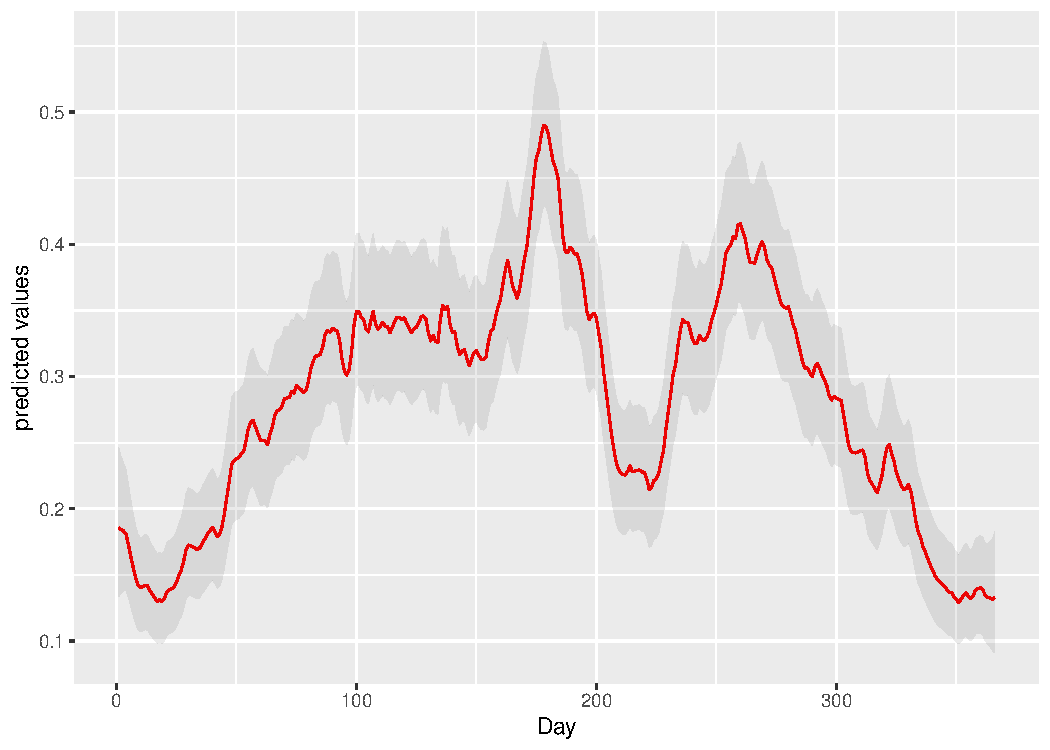
\includegraphics{Exercise-2-ny_files/figure-latex/plot-mod1-1} 

}

\caption{Plot of mean of fitted values of model 1}\label{fig:plot-mod1}
\end{figure}

We see in figure \ref{fig:plot-mod1} that we get a similar graph as in problem 1. We look specifically at \(\pi(\tau_1), \pi(\tau_{201})\) and \(\pi(\tau_{366}).\)

\begin{Shaded}
\begin{Highlighting}[]
\CommentTok{\# pi(tau\_1)}
\NormalTok{mod1}\SpecialCharTok{$}\NormalTok{summary.fitted.values[}\DecValTok{1}\NormalTok{, ]}
\end{Highlighting}
\end{Shaded}

\begin{verbatim}
##                           mean         sd 0.025quant  0.5quant 0.975quant
## fitted.Predictor.001 0.1857515 0.02889715   0.133635 0.1841906  0.2467199
##                           mode
## fitted.Predictor.001 0.1810586
\end{verbatim}

\begin{Shaded}
\begin{Highlighting}[]
\NormalTok{mod1}\SpecialCharTok{$}\NormalTok{summary.fitted.values[}\DecValTok{201}\NormalTok{, ]}
\end{Highlighting}
\end{Shaded}

\begin{verbatim}
##                           mean         sd 0.025quant  0.5quant 0.975quant
## fitted.Predictor.201 0.3329556 0.02871629  0.2785433 0.3322929  0.3911323
##                           mode
## fitted.Predictor.201 0.3309674
\end{verbatim}

\begin{Shaded}
\begin{Highlighting}[]
\NormalTok{mod1}\SpecialCharTok{$}\NormalTok{summary.fitted.values[}\DecValTok{366}\NormalTok{, ]}
\end{Highlighting}
\end{Shaded}

\begin{verbatim}
##                           mean         sd 0.025quant  0.5quant 0.975quant
## fitted.Predictor.366 0.1328162 0.02346736 0.09103365 0.1313649  0.1828461
##                           mode
## fitted.Predictor.366 0.1284723
\end{verbatim}

The computational time according to the proc.time(){[}3{]} is 0.79.

\hypertarget{b-robustness-of-the-results-to-different-control.inla-inputs}{%
\subsection{b) Robustness of the results to different control.inla inputs}\label{b-robustness-of-the-results-to-different-control.inla-inputs}}

We want to look at how robust the results of the two control.inputs are. The strategy we used for integration is ccd. The ccd integration is a less costly alternative compared to the grid strategy when the dimensions of the hyperparameter is large. The grid strategy gives the most accurate result, but the number of points grow exponentially with the dimension of \(\theta.\) The ccd approach locates fewer points around the mode and is therefore less computationally expensive. Other options for integration strategies are `eb', `user' and `user.std'. The `auto' option which is the default integration strategy corresponds with the grid approach if the dimension of \(\theta\) 2 or lower, and ccd if the dimension of \(\theta\) is over 2. We have that the dimension of \(\theta\) is 1, so the auto option will correspond with `grid'.

The default option for strategy is the simplified Laplace option which is the option we have used here. Another option is the Gaussian approximation which is easy to apply and cheap to compute. However, there could be errors in location or due to skeweness. Simplified Laplace can correct these errors and is computationally faster than the Laplace approximation.
This method is therefore regarded as a compromise between accuracy and computational cost. Other options are `adaptive' and `eb'.

We fit a couple of different models with different strategies and compare the results. We start by fitting some models with different integration strategies and the `simplified.laplace' strategy for approximations. The first integration option we use is `grid'.

\begin{Shaded}
\begin{Highlighting}[]
\CommentTok{\# control.inla input}
\NormalTok{control.inla }\OtherTok{=} \FunctionTok{list}\NormalTok{(}\AttributeTok{strategy =} \StringTok{"simplified.laplace"}\NormalTok{, }\AttributeTok{int.strategy =} \StringTok{"grid"}\NormalTok{)}
\CommentTok{\# Fit model}
\NormalTok{fit2 }\OtherTok{\textless{}{-}} \FunctionTok{INLA\_fit}\NormalTok{(control.inla)}
\NormalTok{mod2 }\OtherTok{\textless{}{-}}\NormalTok{ fit2}\SpecialCharTok{$}\NormalTok{mod}
\NormalTok{time2 }\OtherTok{\textless{}{-}}\NormalTok{ fit2}\SpecialCharTok{$}\NormalTok{time}
\end{Highlighting}
\end{Shaded}

We plot the predictions together with the predictions from the first model.

\begin{Shaded}
\begin{Highlighting}[]
\FunctionTok{INLA\_plot\_2}\NormalTok{(mod1, mod2)}
\end{Highlighting}
\end{Shaded}

\begin{figure}

{\centering 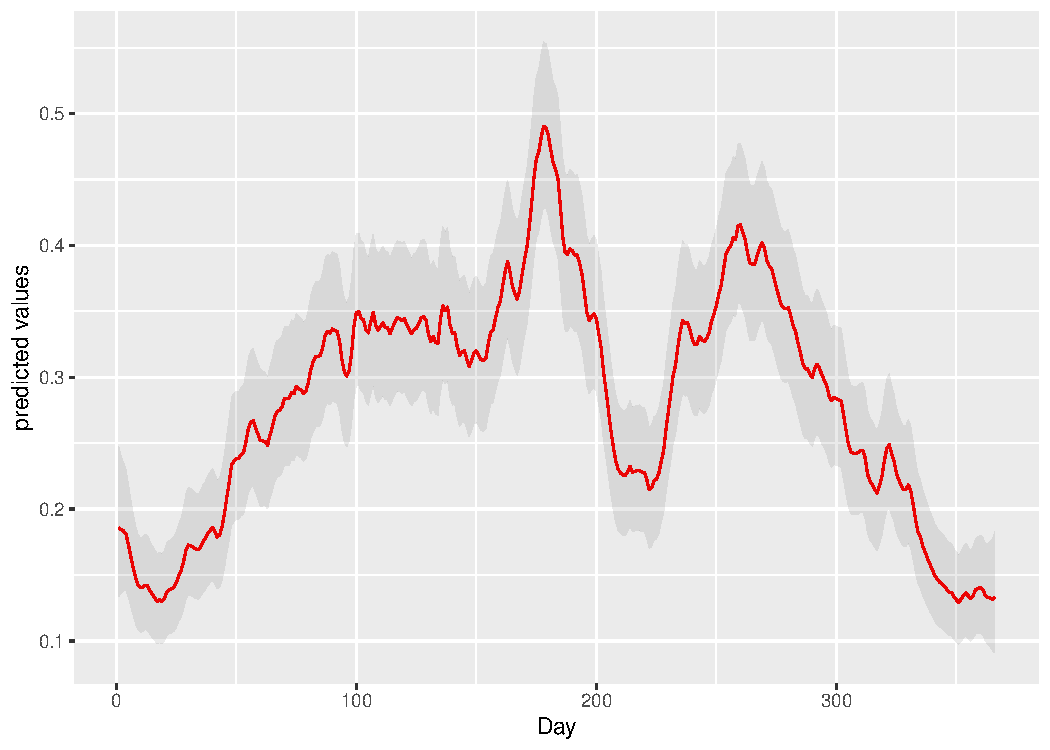
\includegraphics{Exercise-2-ny_files/figure-latex/plot-mod2-1} 

}

\caption{Plot of mean of fitted values of the model with strategy=simplified.laplace and int.strategy=grid compared to plot of model 1}\label{fig:plot-mod2}
\end{figure}

As seen in figure \ref{fig:plot-mod2}, the results from the two models are very similar. The computational time we get by using proc.time(){[}3{]} is 1.03, which is barely higher than the first model.

The next integration strategy considered is the `eb' strategy.

\begin{Shaded}
\begin{Highlighting}[]
\NormalTok{control.inla }\OtherTok{=} \FunctionTok{list}\NormalTok{(}\AttributeTok{strategy =} \StringTok{"simplified.laplace"}\NormalTok{, }\AttributeTok{int.strategy =} \StringTok{"eb"}\NormalTok{)}
\CommentTok{\# Time before}
\NormalTok{fit3 }\OtherTok{\textless{}{-}} \FunctionTok{INLA\_fit}\NormalTok{(control.inla)}
\NormalTok{mod3 }\OtherTok{\textless{}{-}}\NormalTok{ fit3}\SpecialCharTok{$}\NormalTok{mod}
\NormalTok{time3 }\OtherTok{\textless{}{-}}\NormalTok{ fit3}\SpecialCharTok{$}\NormalTok{time}
\end{Highlighting}
\end{Shaded}

We plot it together with the first model

\begin{Shaded}
\begin{Highlighting}[]
\FunctionTok{INLA\_plot\_2}\NormalTok{(mod1, mod3)}
\end{Highlighting}
\end{Shaded}

\begin{figure}

{\centering 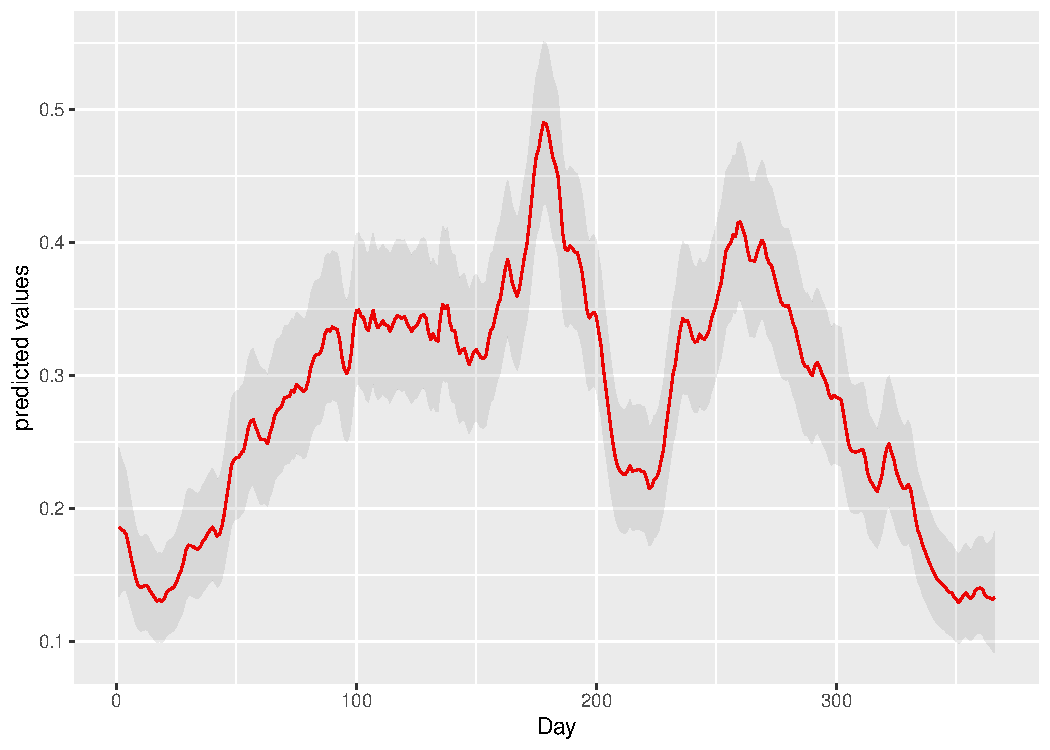
\includegraphics{Exercise-2-ny_files/figure-latex/plot-mod3-1} 

}

\caption{Plot of mean of fitted values of the model with strategy=simplified.laplace and int.strategy=eb compared to plot of model 1}\label{fig:plot-mod3}
\end{figure}

Plot \ref{fig:plot-mod3} shows that this model yields very similar predictions as the two other models.
The computation time is here 0.59, which is about the same as the time when using `grid'. The results for the different integration strategies are very similar. We now look at different strategies for approximation and use ccd as the method for integration strategy. We start by trying the Gaussian approximation.

\begin{Shaded}
\begin{Highlighting}[]
\NormalTok{control.inla }\OtherTok{=} \FunctionTok{list}\NormalTok{(}\AttributeTok{strategy =} \StringTok{"gaussian"}\NormalTok{, }\AttributeTok{int.strategy =} \StringTok{"ccd"}\NormalTok{)}
\NormalTok{fit4 }\OtherTok{\textless{}{-}} \FunctionTok{INLA\_fit}\NormalTok{(control.inla)}
\NormalTok{mod4 }\OtherTok{\textless{}{-}}\NormalTok{ fit4}\SpecialCharTok{$}\NormalTok{mod}
\NormalTok{time4 }\OtherTok{\textless{}{-}}\NormalTok{ fit4}\SpecialCharTok{$}\NormalTok{time}
\end{Highlighting}
\end{Shaded}

\begin{Shaded}
\begin{Highlighting}[]
\FunctionTok{INLA\_plot\_2}\NormalTok{(mod1, mod4)}
\end{Highlighting}
\end{Shaded}

\begin{figure}

{\centering 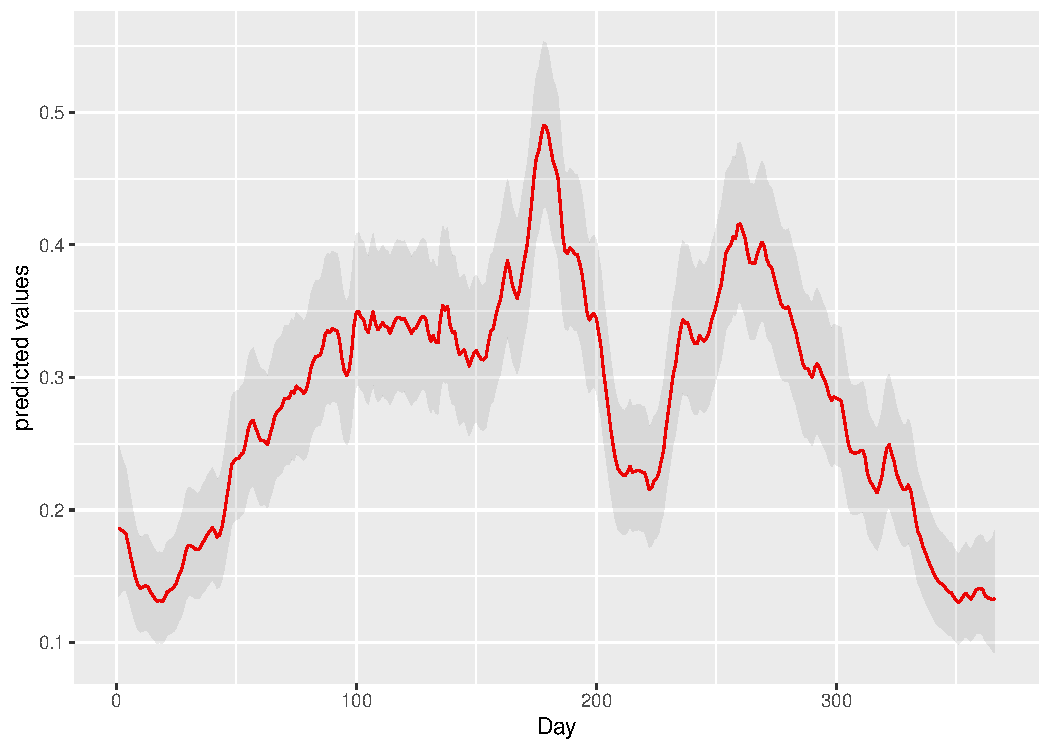
\includegraphics{Exercise-2-ny_files/figure-latex/plot-mod4-1} 

}

\caption{Plot of mean of fitted values of the model with strategy=gaussian and int.strategy=ccd compared to plot of model 1}\label{fig:plot-mod4}
\end{figure}

As seen in \ref{fig:plot-mod4}, we yet again get very similar results. The computation time is 0.59. Now, we use the Laplace approximation.

\begin{Shaded}
\begin{Highlighting}[]
\NormalTok{control.inla }\OtherTok{=} \FunctionTok{list}\NormalTok{(}\AttributeTok{strategy =} \StringTok{"laplace"}\NormalTok{, }\AttributeTok{int.strategy =} \StringTok{"ccd"}\NormalTok{)}
\NormalTok{fit5 }\OtherTok{\textless{}{-}} \FunctionTok{INLA\_fit}\NormalTok{(control.inla)}
\NormalTok{mod5 }\OtherTok{\textless{}{-}}\NormalTok{ fit5}\SpecialCharTok{$}\NormalTok{mod}
\NormalTok{time5 }\OtherTok{\textless{}{-}}\NormalTok{ fit5}\SpecialCharTok{$}\NormalTok{time}
\end{Highlighting}
\end{Shaded}

\begin{Shaded}
\begin{Highlighting}[]
\FunctionTok{INLA\_plot\_2}\NormalTok{(mod1, mod5)}
\end{Highlighting}
\end{Shaded}

\begin{figure}

{\centering 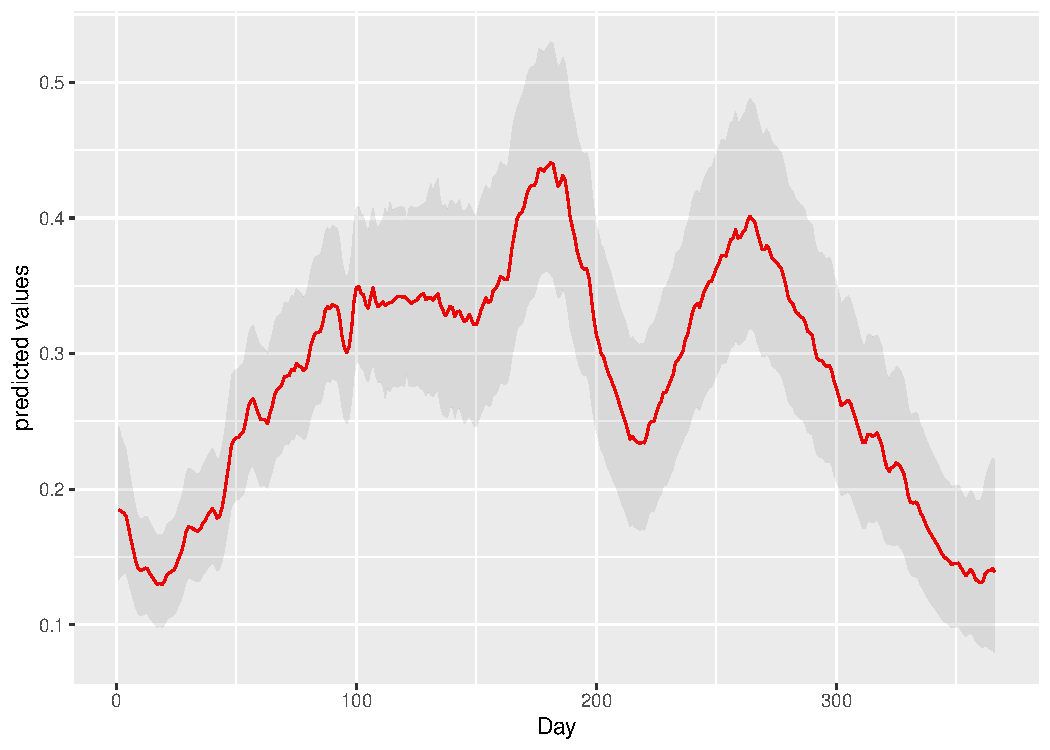
\includegraphics{Exercise-2-ny_files/figure-latex/plot-mod5-1} 

}

\caption{Plot of fitted values with strategy=laplace and int.strategy=ccd compared to model 1}\label{fig:plot-mod5}
\end{figure}

Figure \ref{fig:plot-mod5} shows that for the first days the predictions are very similar. However, from about day 100 and onwards we can see significant differences between the models. The running time is 0.81, which is more compared to the other models.
We also try the Laplace approach with the grid approximation for integration.

\begin{Shaded}
\begin{Highlighting}[]
\NormalTok{control.inla }\OtherTok{=} \FunctionTok{list}\NormalTok{(}\AttributeTok{strategy =} \StringTok{"laplace"}\NormalTok{, }\AttributeTok{int.strategy =} \StringTok{"grid"}\NormalTok{)}
\NormalTok{fit6 }\OtherTok{\textless{}{-}} \FunctionTok{INLA\_fit}\NormalTok{(control.inla)}
\NormalTok{mod6 }\OtherTok{\textless{}{-}}\NormalTok{ fit6}\SpecialCharTok{$}\NormalTok{mod}
\NormalTok{time6 }\OtherTok{\textless{}{-}}\NormalTok{ fit6}\SpecialCharTok{$}\NormalTok{time}
\end{Highlighting}
\end{Shaded}

We compare this to the previous model

\begin{Shaded}
\begin{Highlighting}[]
\FunctionTok{INLA\_plot\_2}\NormalTok{(mod5, mod6)}
\end{Highlighting}
\end{Shaded}

\begin{figure}

{\centering 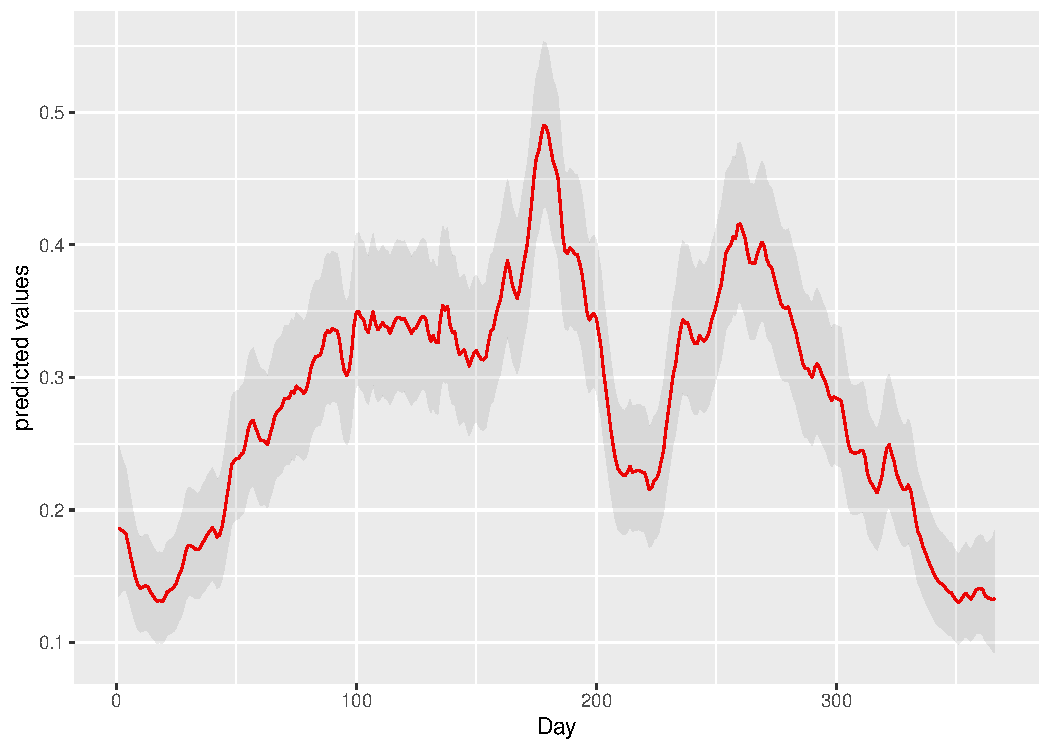
\includegraphics{Exercise-2-ny_files/figure-latex/plot-mod6-1} 

}

\caption{Plot of fitted values with strategy=laplace and int.strategy=grid compared to the values when using strategy=laplace and int.strategy=ccd which is model 5}\label{fig:plot-mod6}
\end{figure}

The predictions are very similar, but we see some differences from about day 100 to day 150. The computation time is 1.03

The Laplace approximation strategy gives different predictions compared to the predictions we get when using other strategies. At last, we look at the `adaptive' strategy and compare it to our original model.

\begin{Shaded}
\begin{Highlighting}[]
\NormalTok{control.inla }\OtherTok{=} \FunctionTok{list}\NormalTok{(}\AttributeTok{strategy =} \StringTok{"adaptive"}\NormalTok{, }\AttributeTok{int.strategy =} \StringTok{"ccd"}\NormalTok{)}
\NormalTok{fit7 }\OtherTok{\textless{}{-}} \FunctionTok{INLA\_fit}\NormalTok{(control.inla)}
\NormalTok{mod7 }\OtherTok{\textless{}{-}}\NormalTok{ fit7}\SpecialCharTok{$}\NormalTok{mod}
\NormalTok{time7 }\OtherTok{\textless{}{-}}\NormalTok{ fit7}\SpecialCharTok{$}\NormalTok{time}
\end{Highlighting}
\end{Shaded}

We compare the predictions of this model to the predictions of the first model.
The running time for fitting this model is 0.59.

The different inputs for control.inla mostly yields very similar results. However, we get different results when using the Laplace approximation as strategy. This imply that the results are not that robust for the different control.inla inputs we use. We also notice a longer running time when using Laplace for approximations. The running time is also larger when using \texttt{grid} compared to the other integrartion strategies. All these running times are all very low compared to our previous results from problem 1.

\hypertarget{c-inla-model-2}{%
\subsection{c) INLA model 2}\label{c-inla-model-2}}

We fit a new model that is fitted with the code below. We refer to this model as model 8.

\begin{Shaded}
\begin{Highlighting}[]
\NormalTok{alpha }\OtherTok{=} \DecValTok{2}
\NormalTok{beta }\OtherTok{=} \FloatTok{0.05}
\NormalTok{hyper }\OtherTok{=} \FunctionTok{list}\NormalTok{(}\AttributeTok{theta =} \FunctionTok{list}\NormalTok{(}\AttributeTok{prior =} \StringTok{"loggamma"}\NormalTok{, }\AttributeTok{param =} \FunctionTok{c}\NormalTok{(alpha, beta)))}
\NormalTok{control.inla }\OtherTok{=} \FunctionTok{list}\NormalTok{(}\AttributeTok{strategy =} \StringTok{"simplified.laplace"}\NormalTok{, }\AttributeTok{int.strategy =} \StringTok{"ccd"}\NormalTok{)}

\NormalTok{mod8 }\OtherTok{\textless{}{-}} \FunctionTok{inla}\NormalTok{(n.rain }\SpecialCharTok{\textasciitilde{}} \FunctionTok{f}\NormalTok{(day, }\AttributeTok{model =} \StringTok{"rw1"}\NormalTok{, }\AttributeTok{hyper =}\NormalTok{ hyper, }\AttributeTok{constr =} \ConstantTok{TRUE}\NormalTok{), }\AttributeTok{data =}\NormalTok{ rain,}
    \AttributeTok{Ntrials =}\NormalTok{ n.years, }\AttributeTok{control.compute =} \FunctionTok{list}\NormalTok{(}\AttributeTok{config =} \ConstantTok{TRUE}\NormalTok{), }\AttributeTok{family =} \StringTok{"binomial"}\NormalTok{,}
    \AttributeTok{verbose =} \ConstantTok{TRUE}\NormalTok{, }\AttributeTok{control.inla =}\NormalTok{ control.inla)}
\end{Highlighting}
\end{Shaded}

The model in problem 2a is has a response given by equation \eqref{eq:1response}.
The first mathematical difference of the new model compared to the first model is that the intercept is not removed. This means that the response is given by

\[
y_t | \eta_t \sim \text{Bin}(n_t, \pi(\eta_t)), \ \ \pi(\eta_t)=\frac{\exp(\eta_t)}{1+\exp(\eta_t)}=\frac{1}{1+\exp(-\eta_t)},
\]
where \(\eta_t=\beta_0+\tau_t,\) and \(\beta_0\) is the intercept. We use the default prior on the intercept which is a Gaussian distribution with the mean and precision equal to zero. This is an improper prior where the variance is infinite. The prior on \(\theta\) is the same as in the model in 2a, that is a \(\text{Loggamma}(\alpha=2, \beta=0.05)-\) distribution.
Unlike the previous model, this model uses the argument \texttt{constr=TRUE}.
This means that there is a sum-to-zero constraint, and the sum of \((\tau_1,..,\tau_n)\) is given by
\[
\sum_{i=1}^{n} \tau_i=0.
\]
We fit the model and compare it to the model from 2a. In the model 8, we have that \(\eta_t\) is given by
\[
\eta_t=\log \left (\frac{\pi (\eta_t)}{1- \pi (\eta_t)} \right) \implies \tau_t=\log \left (\frac{\pi (\eta_t)}{1- \pi (\eta_t)} \right)-\alpha
\]
In the model in 2a, we have

\[
\tau_t=\log \left (\frac{\pi (\tau_t)}{1- \pi (\tau_t)} \right) 
\]
Below, we plot the estimated mean values of \(\tau_t\) for \(t=1,..,T\) for both models.

\begin{Shaded}
\begin{Highlighting}[]
\NormalTok{tau\_1 }\OtherTok{=}\NormalTok{ mod1}\SpecialCharTok{$}\NormalTok{summary.random}\SpecialCharTok{$}\NormalTok{day}\SpecialCharTok{$}\NormalTok{mean}
\NormalTok{tau\_8 }\OtherTok{=}\NormalTok{ mod8}\SpecialCharTok{$}\NormalTok{summary.random}\SpecialCharTok{$}\NormalTok{day}\SpecialCharTok{$}\NormalTok{mean}
\NormalTok{label1 }\OtherTok{=} \FunctionTok{c}\NormalTok{(}\StringTok{"Model 1"}\NormalTok{, }\StringTok{"Model 8"}\NormalTok{)}
\FunctionTok{ggplot}\NormalTok{() }\SpecialCharTok{+} \FunctionTok{geom\_line}\NormalTok{(}\AttributeTok{data =} \FunctionTok{as.data.frame}\NormalTok{(tau\_1), }\AttributeTok{mapping =} \FunctionTok{aes}\NormalTok{(}\AttributeTok{x =} \DecValTok{1}\SpecialCharTok{:}\DecValTok{366}\NormalTok{, }\AttributeTok{y =}\NormalTok{ tau\_1,}
    \AttributeTok{color =} \StringTok{"Model 1"}\NormalTok{)) }\SpecialCharTok{+} \FunctionTok{geom\_line}\NormalTok{(}\AttributeTok{data =} \FunctionTok{as.data.frame}\NormalTok{(tau\_8), }\AttributeTok{mapping =} \FunctionTok{aes}\NormalTok{(}\AttributeTok{x =} \DecValTok{1}\SpecialCharTok{:}\DecValTok{366}\NormalTok{,}
    \AttributeTok{y =}\NormalTok{ tau\_8, }\AttributeTok{color =} \StringTok{"model 8"}\NormalTok{)) }\SpecialCharTok{+} \FunctionTok{xlab}\NormalTok{(}\StringTok{"Day"}\NormalTok{) }\SpecialCharTok{+} \FunctionTok{ylab}\NormalTok{(}\StringTok{"estimated values of"} \SpecialCharTok{\textasciitilde{}}\NormalTok{ tau) }\SpecialCharTok{+}
    \FunctionTok{labs}\NormalTok{(}\AttributeTok{color =} \StringTok{"Models"}\NormalTok{)}
\end{Highlighting}
\end{Shaded}

\begin{figure}

{\centering 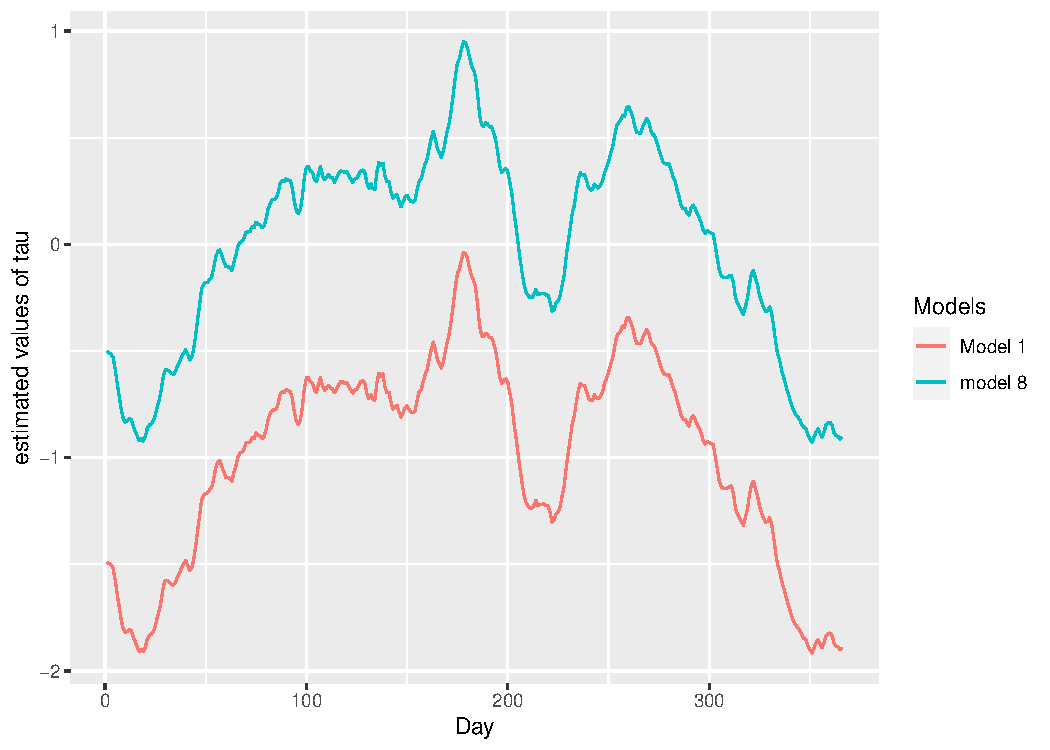
\includegraphics{Exercise-2-ny_files/figure-latex/plot-2c-tau-1} 

}

\caption{$\tau$-values of model 1 and 8}\label{fig:plot-2c-tau}
\end{figure}

As seen in figure \ref{fig:plot-2c-tau}, the predicted \(\tau\)-values are different for the two models. The model
with the intercept and sum-to-zero constraint is supposed to have tau-values that sum to zero, and
from the figure it seems like that this is the case. The model without the intercept does not have tauvalues that sums to zero as seen in the figure. Nevertehelss, we can see that the to graphs have what seems like identical shapes.
The predicted \(\pi-\)values of the models in 2a and 2c are also plotted together.

\begin{Shaded}
\begin{Highlighting}[]
\FunctionTok{ggplot}\NormalTok{() }\SpecialCharTok{+} \FunctionTok{geom\_line}\NormalTok{(}\AttributeTok{data =} \FunctionTok{as.data.frame}\NormalTok{(mod1}\SpecialCharTok{$}\NormalTok{summary.fitted.values}\SpecialCharTok{$}\NormalTok{mean), }\AttributeTok{mapping =} \FunctionTok{aes}\NormalTok{(}\AttributeTok{x =} \DecValTok{1}\SpecialCharTok{:}\DecValTok{366}\NormalTok{,}
    \AttributeTok{y =}\NormalTok{ mod1}\SpecialCharTok{$}\NormalTok{summary.fitted.values}\SpecialCharTok{$}\NormalTok{mean, }\AttributeTok{color =} \StringTok{" Model 1"}\NormalTok{), }\AttributeTok{color =} \StringTok{"black"}\NormalTok{) }\SpecialCharTok{+}
    \FunctionTok{geom\_line}\NormalTok{(}\AttributeTok{data =} \FunctionTok{as.data.frame}\NormalTok{(mod8}\SpecialCharTok{$}\NormalTok{summary.fitted.values}\SpecialCharTok{$}\NormalTok{mean), }\AttributeTok{mapping =} \FunctionTok{aes}\NormalTok{(}\AttributeTok{x =} \DecValTok{1}\SpecialCharTok{:}\DecValTok{366}\NormalTok{,}
        \AttributeTok{y =}\NormalTok{ mod8}\SpecialCharTok{$}\NormalTok{summary.fitted.values}\SpecialCharTok{$}\NormalTok{mean, }\AttributeTok{color =} \StringTok{" Model 2"}\NormalTok{), }\AttributeTok{color =} \StringTok{"red"}\NormalTok{) }\SpecialCharTok{+}
    \FunctionTok{xlab}\NormalTok{(}\StringTok{"Day"}\NormalTok{) }\SpecialCharTok{+} \FunctionTok{ylab}\NormalTok{(}\StringTok{"Fitted values"}\NormalTok{) }\SpecialCharTok{+} \FunctionTok{labs}\NormalTok{(}\StringTok{"Models"}\NormalTok{)}
\end{Highlighting}
\end{Shaded}

\begin{figure}

{\centering 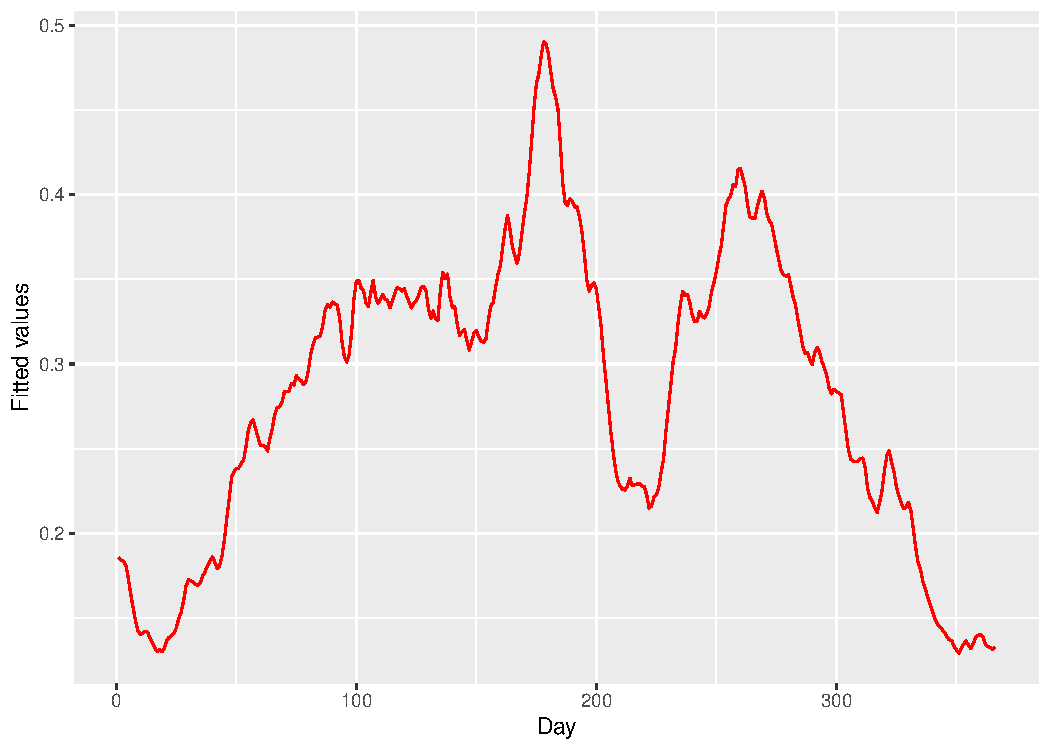
\includegraphics{Exercise-2-ny_files/figure-latex/plot-2c-1} 

}

\caption{Fitted values of model 1 and 8}\label{fig:plot-2c}
\end{figure}

From figure \ref{fig:plot-2c} we can't see any significant differences. The estimated values of the mean of \(\pi(\tau_1)\), \(\pi(\tau_{201})\) and \(\pi (\tau_{366})\) is printed below.

\begin{Shaded}
\begin{Highlighting}[]
\NormalTok{mod8}\SpecialCharTok{$}\NormalTok{summary.fitted.values[}\DecValTok{1}\NormalTok{, ]}
\end{Highlighting}
\end{Shaded}

\begin{verbatim}
##                           mean         sd 0.025quant  0.5quant 0.975quant
## fitted.Predictor.001 0.1857527 0.02889691  0.1336365 0.1841919  0.2467204
##                         mode
## fitted.Predictor.001 0.18106
\end{verbatim}

\begin{Shaded}
\begin{Highlighting}[]
\NormalTok{mod8}\SpecialCharTok{$}\NormalTok{summary.fitted.values[}\DecValTok{201}\NormalTok{, ]}
\end{Highlighting}
\end{Shaded}

\begin{verbatim}
##                           mean         sd 0.025quant  0.5quant 0.975quant
## fitted.Predictor.201 0.3329546 0.02871596  0.2785427 0.3322919  0.3911304
##                           mode
## fitted.Predictor.201 0.3309666
\end{verbatim}

\begin{Shaded}
\begin{Highlighting}[]
\NormalTok{mod8}\SpecialCharTok{$}\NormalTok{summary.fitted.values[}\DecValTok{366}\NormalTok{, ]}
\end{Highlighting}
\end{Shaded}

\begin{verbatim}
##                           mean         sd 0.025quant  0.5quant 0.975quant
## fitted.Predictor.366 0.1328184 0.02346735 0.09103599 0.1313672  0.1828485
##                           mode
## fitted.Predictor.366 0.1284745
\end{verbatim}

\begin{Shaded}
\begin{Highlighting}[]
\NormalTok{intercept }\OtherTok{\textless{}{-}}\NormalTok{ mod8}\SpecialCharTok{$}\NormalTok{summary.fixed}\SpecialCharTok{$}\NormalTok{mean}
\end{Highlighting}
\end{Shaded}

To further show how similar the predictions are, we can look at \(\pi\) for day 1, 201 and 366.
These predictions are very similar, and the first differences can be seen in the fith decimal.

The estimated intercept term is -0.9876664.

We see that the estimated \(\tau\) values are different between the two models. The reason for this is as stated that there is a sum-to-zero constraint on the second model. However, the shape of the graphs are similar. The intercept term makes up for the fact that there are different constraints and we get very similar results. This can also be seen when calculating the posterior distribution.

\end{document}
